% فصل ۳
\chapter{روش‌شناسی و معماری پیشنهادی}\label{chap:methodology}


% -----------------------------------------------------------------------
\section{رویکرد کلی پژوهش}\label{sec:method-approach}

بررسی پژوهش‌های پیشین در فصل دوم نشان داد که حوزه پیش‌بینی \gls{RUL} و پایش تجهیزات صنعتی با چند شکاف بنیادین روبه‌روست. نبود چارچوبی یکپارچه که \glspl{MAS}، \glspl{Digital Twins} و \glspl{LLM} را در یک معماری منسجم ترکیب کند؛ غفلت از توضیح‌پذیری نتایج پیش‌بینی و نقش حسگرهای مختلف در تصمیم مدل و بی‌توجهی به هزینه نامتقارن خطای بیش‌برآورد در \gls{predictive maintenance}. این فصل پاسخ روش‌شناختی پژوهش حاضر به این شکاف‌ها را ارائه می‌دهد.

روش‌شناسی پژوهش حاضر به صورت خطی و یک مرحله‌ای نیست. پس از بررسی پژوهش‌های مرتبط در حوزه دوقلوی دیجیتال، \glspl{MAS} و کاربردهای صنعتی، کار در دو شاخه ادامه می‌یابد. شاخه نخست به انتخاب مجموعه داده \gls{CMAPSS} و سپس مرور پژوهش‌های تازه‌تر --- از جمله پیش‌بینی \gls{RUL} با \gls{LSTM} و ادغام \gls{LLM} با دوقلوهای دیجیتال --- می‌پردازد. شاخه دوم معماری پنج‌لایه چندعاملی را طراحی می‌کند. این دو شاخه در شناسایی شکاف‌ها به هم می‌رسند تا معماری پیشنهادی به مسائل موجود در شکاف‌های شناسایی شده پاسخ دهد. نبود سامانه و معماری یکپارچه دوقلوی دیجیتال، ضعف توضیح‌پذیری توسط حسگر‌ها و هزینه نامتقارن خطا در پیش‌بینی مجموعه‌داده \gls{CMAPSS} از جمله آن مسائل است. پس از آن، نمونه‌سازی آزمایشگاهی و ارزیابی تجربی انجام می‌شود. شکل \ref{fig:method-flow} این مسیر هفت مرحله‌ای را نشان می‌دهد.


در سمت چپ شکل \ref{fig:method-flow}، انتخاب \gls{CMAPSS} مرور ادبیات را به کارهای مسئله‌محور محدود می‌کند که شامل پژوهش‌های متنوع در زمینه این مجموعه داده است. در سمت راست، ادبیات پایه‌ای به طراحی مفهومی لایه‌ها، عامل‌ها و \gls{Protocol} تعامل می‌پردازد. نقطه تلاقی این دو شاخه مرحله شکاف‌هاست. معماری باید یکپارچگی چندعاملی، توضیح سهم حسگرها و سوگیری آگاهانه به کم‌برآورد را پوشش دهد. مرحله ششم این طراحی را روی داده شبیه‌سازی‌شده پیاده می‌کند و سطح بلوغ هدف را از \gls{DTSH} یک‌طرفه به \gls{Digital Twins} با ارتباط \gls{Bidirectional} در بستر شبیه‌سازی می‌رساند \cite{tao2019digital}. مرحله پایانی معیارهای کمی پیش‌بینی، نسبت خطای کم‌برآورد و کیفیت توضیح عامل زبانی را ارائه می‌دهد.


در خصوص هزینه نامتقارن خطا، پژوهش حاضر رویکردی متمایز دارد. در \gls{predictive maintenance}، بیش‌برآورد \gls{RUL} --- یعنی پیش‌بینی بیشتر از عمر واقعی تجهیز --- می‌تواند باعث خرابی ناگهانی و ایجاد هزینه قابل توجه شود. در مقابل، کم‌برآورد عمر، اگرچه ممکن است بررسی تجهیز را زود‌تر از زمان واقعی، پیشنهاد دهد اما خطر خرابی را به‌شدت کاهش می‌دهد. بنابراین پژوهش حاضر تابع هزینه‌ای طراحی می‌کند که خطاها را آگاهانه به سمت کم‌برآورد سوق می‌دهد. به این معنا که اگر مدل در پیش‌بینی اشتباه کند، عمر باقیمانده را کمتر از واقعیت برآورد می‌کند، نه بیشتر. این انتخاب آگاهانه، یک انتخاب محافظه‌کارانه و ایمن در فرآیندهای صنعتی واقعی است.


\begin{figure}[H]
	\centering
	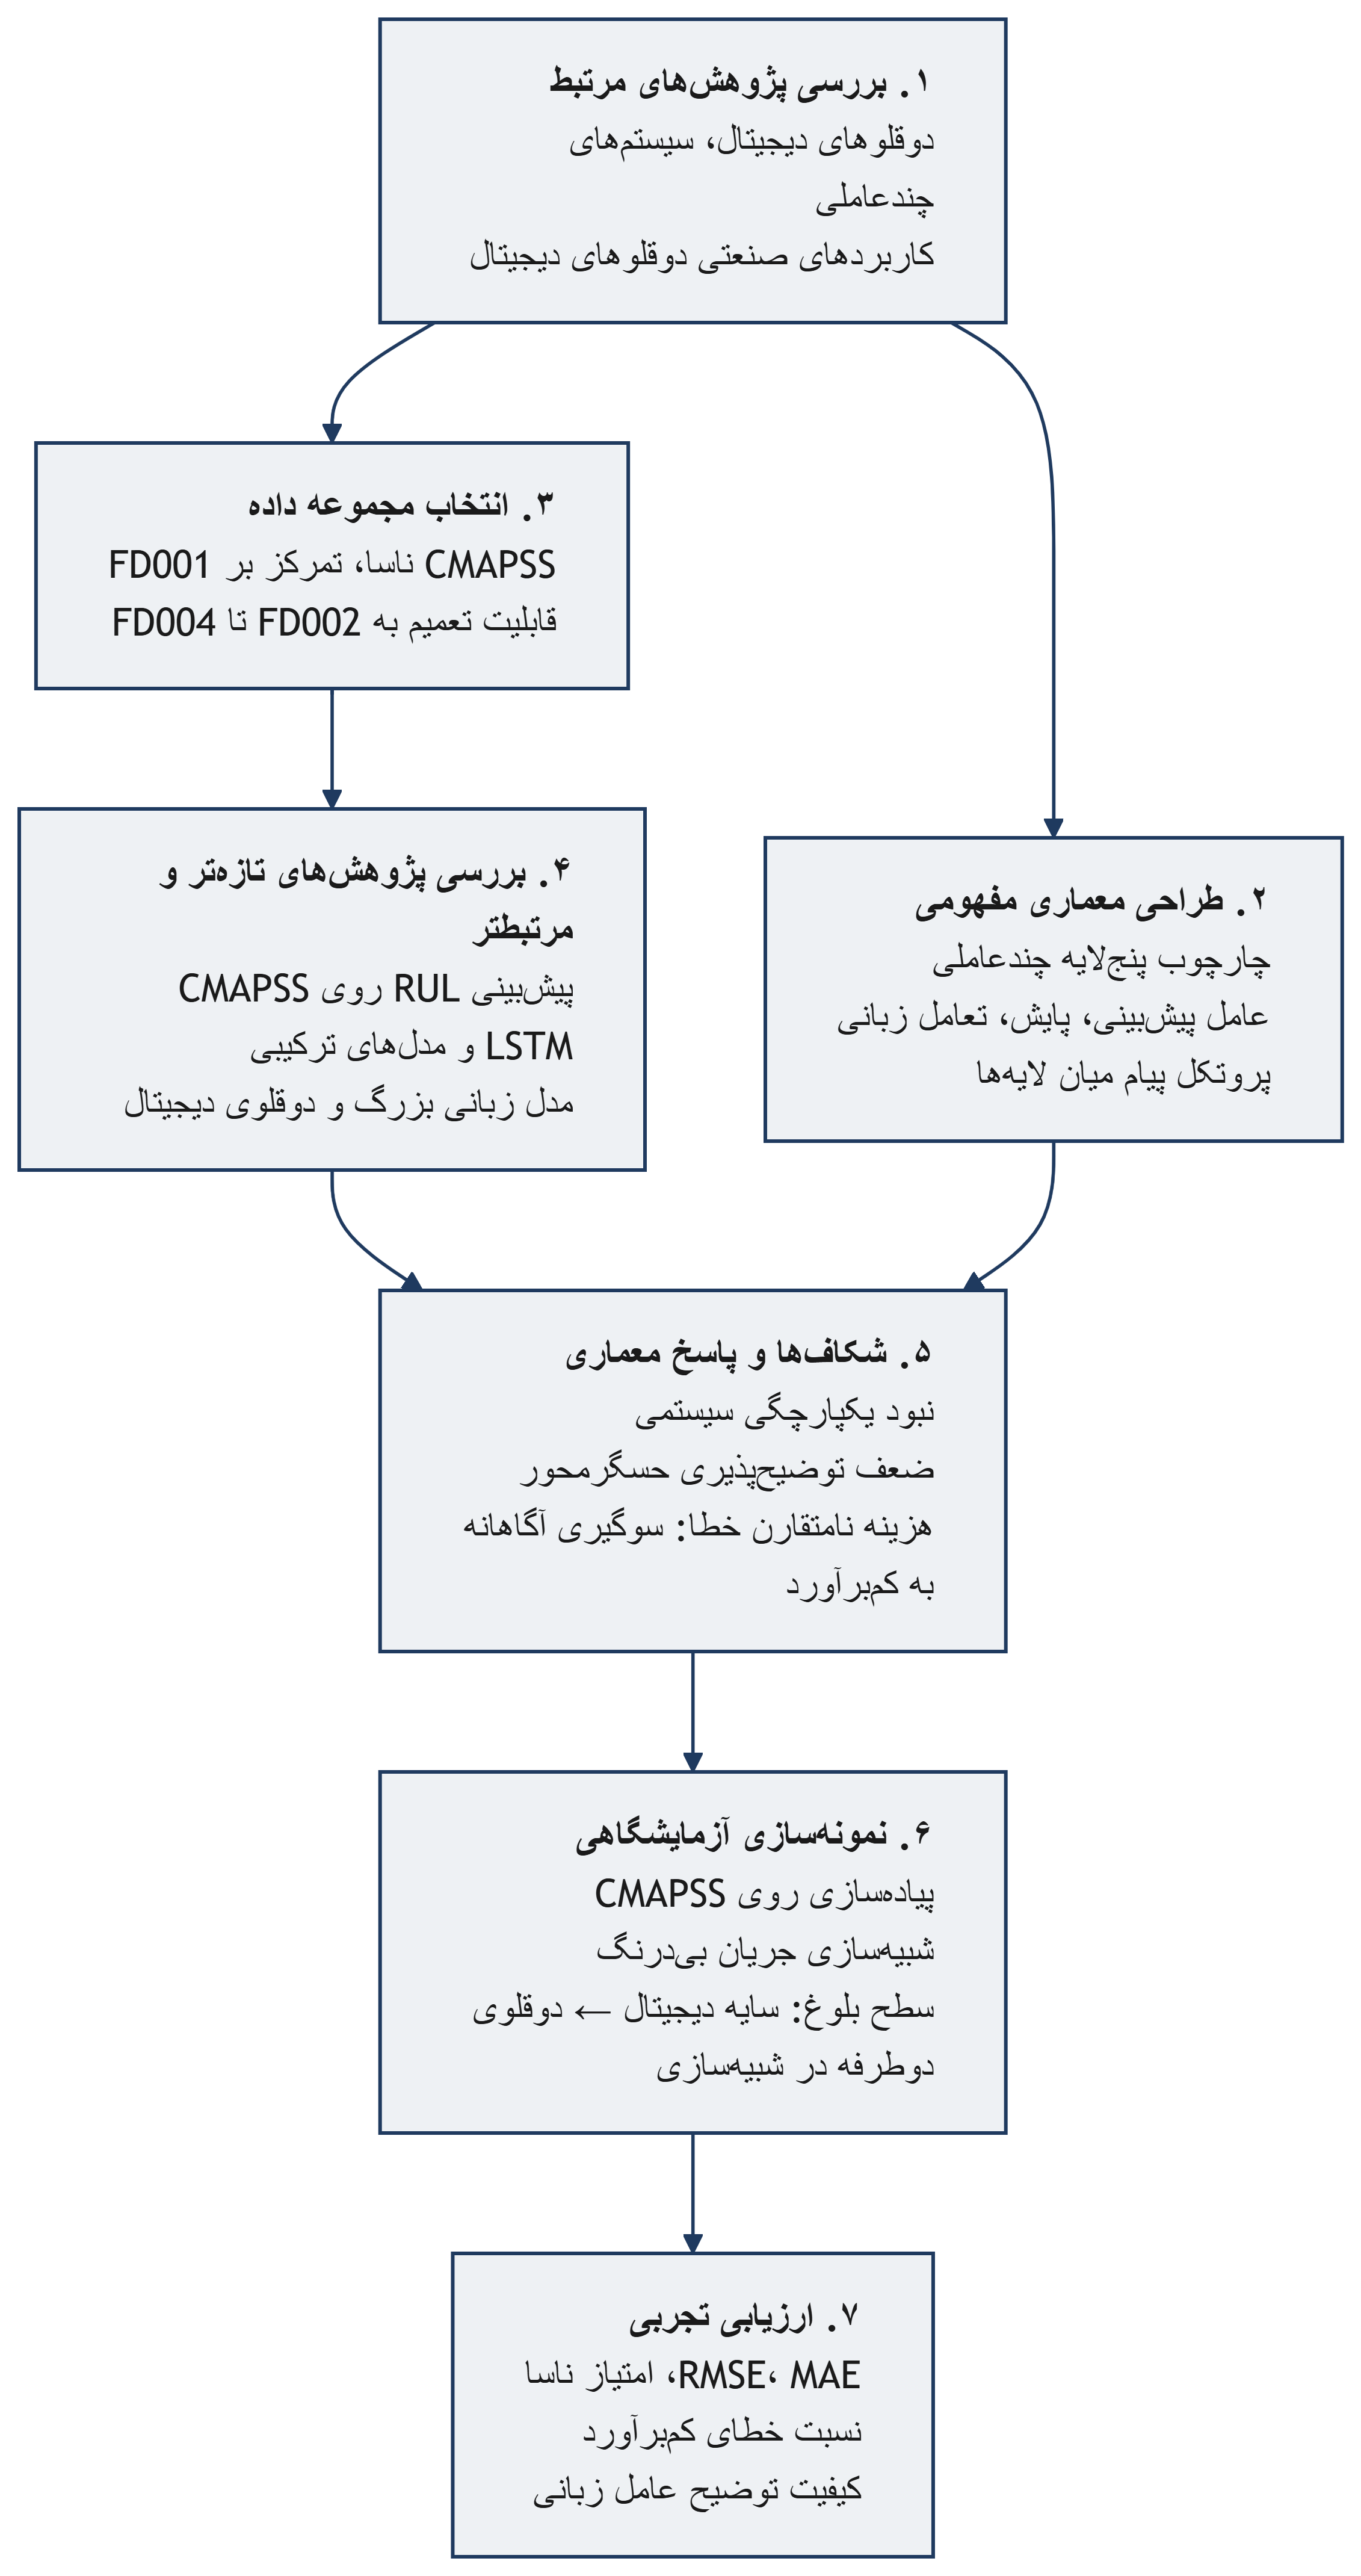
\includegraphics[width=0.8\textwidth]{images/method_flow.png}
	\caption{
		مسیر هفت‌ مرحله‌ای پژوهش که پس از بررسی پژوهش‌های مرتبط، دو شاخه موازی  می‌شود و انتخاب داده به همراه طراحی معماری پیش می‌رود. در شناسایی شکاف‌ها به هم می‌رسند و در نهایت ارزیابی صورت می‌گیرد.}
	\label{fig:method-flow}
\end{figure}


% -----------------------------------------------------------------------


% -----------------------------------------------------------------------
\section{معماری پیشنهادی دوقلوی دیجیتال چندعاملی}
\label{sec:architecture}

\subsection{نمای کلی و اصول طراحی}
\label{sec:arch-overview}

معماری پیشنهادی این پژوهش، یک چارچوب پنج‌لایه برای پیاده‌سازی \gls{MA-DT} در سامانه‌های پایش و نگهداری پیش‌بینانه است که با هدف ایجاد یک زنجیره یکپارچه از موجودیت فیزیکی تا تصمیم‌گیری سطح‌بالا طراحی شده است. ایده اصلی معماری آن است که داده‌های تولیدشده توسط موجودیت فیزیکی، پس از جمع‌آوری و آماده‌سازی، در یک لایه دیجیتال متشکل از عامل‌های دوقلوی دیجیتال بازنمایی شوند و سپس عامل‌های کاربردی بتوانند بر مبنای وضعیت جاری این دوقلوها، وظایفی نظیر پیش‌بینی \gls{RUL}، پایش وضعیت، تشخیص، زمان‌بندی نگهداری و تعامل زبانی با کاربر را انجام دهند. چنین تفکیکی با دیدگاه‌های کلاسیک درباره دوقلوی دیجیتال که بر پیوند دوسویه میان موجودیت فیزیکی و بازنمایی دیجیتال، همگام‌سازی وضعیت و استفاده از داده‌های بی‌درنگ تأکید دارند، سازگار است \cite{tao2019digital,barricelli2019survey,fuller2020digital,qi2021enabling}. در عین حال، استفاده از معماری چندعاملی امکان می‌دهد که پیچیدگی سامانه به مجموعه‌ای از واحدهای خودمختار اما هماهنگ تقسیم شود؛ به‌گونه‌ای که هر عامل مسئولیت مشخصی را بر عهده داشته باشد و از طریق قراردادهای ارتباطی تعریف‌شده با سایر عامل‌ها همکاری کند \cite{dorri2018multiagent,pretel2022masdt,lopez2024madtwin,wang2024multiagent}.

معماری حاضر از پنج لایه اصلی شامل \gls{EmtityLayer}، \gls{DataCollectionLayer}، \gls{IntegrationLayer}، \gls{DigitalTwinAgentsLayer} و \gls{ApplicationAgentsLayer} تشکیل شده است. این پنج لایه را می‌توان در سه فضای مفهومی بزرگ‌تر نیز دسته‌بندی کرد: لایه موجودیت در فضای فیزیکی، لایه‌های جمع‌آوری و ادغام در فضای ارتباطی و دو لایه عامل‌های دوقلوی دیجیتال و عامل‌های کاربرد در فضای دیجیتال. این تفکیک با رویکردهای معماری دوقلوی دیجیتال که مرز میان موجودیت فیزیکی، جریان داده، مدل دیجیتال و خدمات کاربردی را مشخص می‌کنند هم‌راستا است \cite{tao2019digital,qi2021enabling}. علاوه بر این، دوقلوهای دیجیتال مجهز به هوش مصنوعی در حال گذار از بازنمایی‌های صرفاً توصیفی به سامانه‌هایی هستند که قادر به پایش، پیش‌بینی، مداخله و در نهایت مدیریت خودکار می‌باشند. در این گذار، مدل‌های یادگیری ماشین و یادگیری عمیق، عامل‌های هوشمند و مدل‌های زبانی بزرگ می‌توانند در لایه‌های متفاوت چرخه عمر دوقلوی دیجیتال قرار گیرند \cite{zhou2026dtai,fu2026genaidt}. پس در معماری پیشنهادی، مدل زبان بزرگ به‌عنوان جایگزین مدل تخصصی پیش‌بینی \gls{RUL} در نظر گرفته نمی‌شود، بلکه در لایه کاربرد و تعامل به‌عنوان یک بخش استدلالی و زبانی مورد استفاده قرار می‌گیرد. این تفکیک سبب می‌شود که محاسبه عددی \gls{RUL} توسط یک مدل تخصصی و قابل ارزیابی مانند LSTM انجام شود و مدل زبان طبیعی بر روی وضعیت ساختاریافته تولیدشده توسط دوقلوی دیجیتال، وظایف تفسیر، ترکیب اطلاعات، پاسخ‌گویی و هدایت عامل‌ها را انجام دهد. چنین تفکیکی با جهت‌گیری پژوهش‌های جدید در زمینه ادغام مدل‌های زبانی بزرگ و دوقلو‌های دیجیتال نیز سازگار است که نقش مدل زبانی بزرگ را در تعامل، ساخت دانش، استدلال و ارائه خدمات سطح‌بالا تعریف می‌شود \cite{CHEN2025102982LLMDT,zhou2026dtai,maghanaki2026llmmanufacturing}.

سه اصل اساسی در طراحی این معماری عبارت‌اند از جداسازی مسئولیت‌ها، استقلال و همکاری عامل‌ها، و مقیاس‌پذیری. اصل نخست بیان می‌کند که دریافت داده، آماده‌سازی داده، نگهداری وضعیت دوقلوی دیجیتال، پیش‌بینی و تعامل با کاربر نباید در یک بخش واحد ادغام شوند؛ زیرا چنین ادغامی باعث افزایش وابستگی متقابل، دشواری آزمون و کاهش قابلیت جایگزینی اجزای سامانه می‌شود. در معماری پیشنهادی، لایه جمع‌آوری صرفاً مسئول دریافت داده است، لایه ادغام مسئول تبدیل داده خام به اطلاعات قابل استفاده، لایه عامل‌های دوقلوی دیجیتال مسئول نگهداری وضعیت دیجیتال موجودیت و لایه عامل‌های کاربرد مسئول ارائه خدمات هوشمند است. اصل دوم از مبانی سامانه‌های چندعاملی ناشی می‌شود. عامل‌ها باید بتوانند به‌صورت مستقل تصمیم‌های محلی خود را بگیرند، اما برای انجام وظایف پیچیده‌تر از طریق پیام‌های استاندارد با یکدیگر همکاری کنند \cite{dorri2018multiagent,pretel2022masdt}. اصل سوم نیز تضمین می‌کند که افزایش تعداد موتورهای تحت پایش یا افزودن خدمات جدید، الزاماً نیازمند بازطراحی لایه‌های پایین‌تر نباشد. این ویژگی به‌خصوص در سامانه‌های دارای تعداد زیادی موجودیت فیزیکی اهمیت دارد و در چارچوب‌های دوقلو‌های دیجیتال چندعاملی نیز به‌عنوان یکی از مزایای اصلی، تفکیک عامل‌ها مطرح شده است \cite{lopez2024madtwin,wang2024multiagent}.

شکل \ref{fig:arch-5layers} نمای کلی معماری پنج‌لایه پیشنهادی را نشان می‌دهد. همان‌گونه که در شکل مشاهده می‌شود، جریان اصلی داده از موجودیت فیزیکی به سمت لایه‌های دیجیتال و کاربردی حرکت می‌کند، در حالی که درخواست‌ها، سیاست‌های کنترلی و فرمان‌های سطح‌بالا می‌توانند در جهت معکوس حرکت کنند. بنابراین، معماری ماهیتی دوطرفه دارد و دوقلوی دیجیتال صرفاً یک مخزن داده یا تصویر ایستا از تجهیز فیزیکی نیست بلکه واسطی برای ایجاد ارتباط میان وضعیت واقعی موجودیت، مدل دیجیتال، خدمات تحلیلی و تصمیم‌های سطح‌بالا محسوب می‌شود \cite{tao2019digital,fuller2020digital,qi2021enabling}.

\begin{figure}[H]
    \centering
    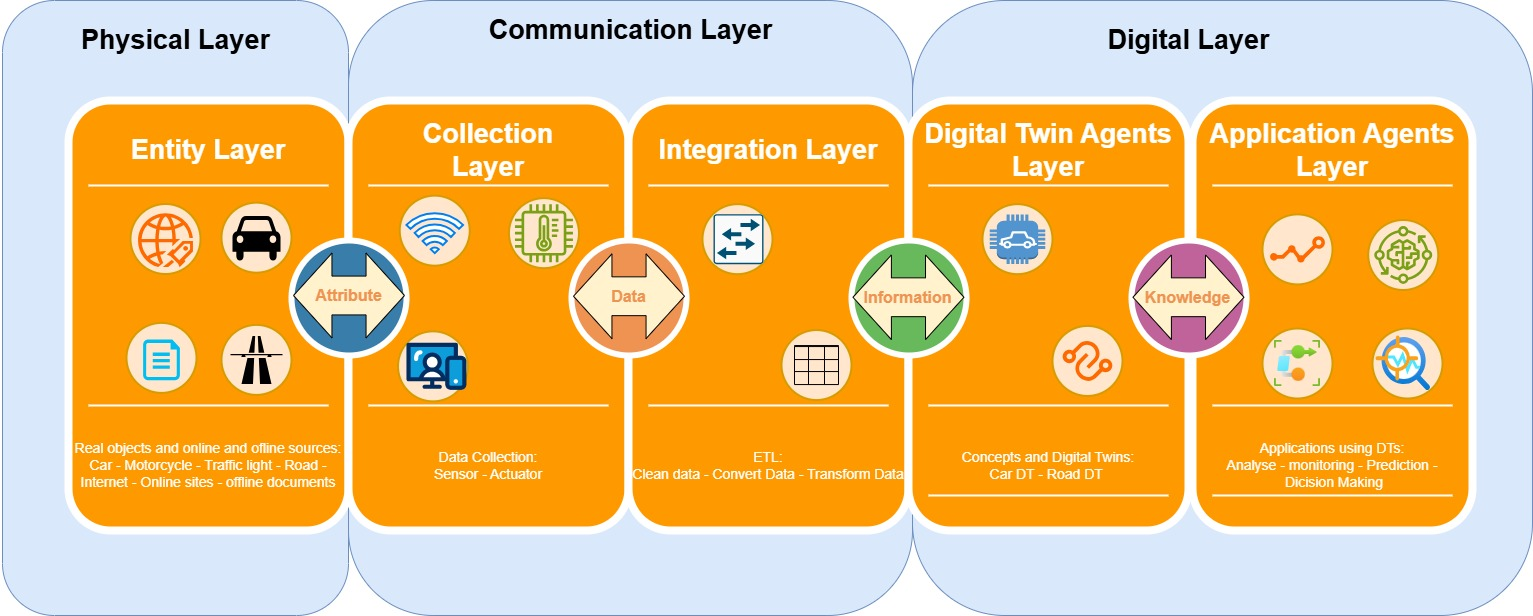
\includegraphics[width=0.98\textwidth]{images/DigitalTwin-Page-4.jpg}
    \caption{معماری پنج‌لایه پیشنهادی دوقلو‌های دیجیتال چندعاملی؛ لایه‌های موجودیت، جمع‌آوری، ادغام، عامل‌های دوقلوی دیجیتال و عامل‌های کاربرد، جریان صعودی داده و جریان نزولی فرمان و بازخورد را تشکیل می‌دهند.}
    \label{fig:arch-5layers}
\end{figure}


\subsection{لایه موجودیت}
\label{sec:layer-entity}

\gls{EmtityLayer} پایین‌ترین لایه معماری و نقطه اتصال سامانه دیجیتال به جهان فیزیکی است. این لایه شامل تجهیز یا فرآیند واقعی مورد مطالعه، حسگرها، عملگرها و سایر مؤلفه‌هایی است که وضعیت فیزیکی سیستم را تعیین می‌کنند. در چارچوب دوقلوی دیجیتال، وجود این موجودیت فیزیکی به‌تنهایی کافی نیست، بلکه باید ارتباطی پایدار میان وضعیت آن و بازنمایی دیجیتال برقرار شود تا تغییرات موجودیت واقعی بتواند در مدل دیجیتال بازتاب شود و در صورت وجود مسیر کنترلی، تصمیم‌های حاصل از فضای دیجیتال نیز به موجودیت فیزیکی منتقل شوند \cite{tao2019digital,barricelli2019survey,fuller2020digital}.
 از این دید، لایه موجودیت را می‌توان منشأ تولید داده در سامانه دانست؛ زیرا داده‌های مربوط به چرخه کاری، وضعیت حسگرها و رویدادهای عملیاتی از همین لایه وارد زنجیره پردازش می‌شوند. در کاربرد مورد نظر این پژوهش، هر موتور هواپیما به‌عنوان یک موجودیت فیزیکی مستقل در نظر گرفته می‌شود و مجموعه‌ای از متغیرها و شاخص‌های آن موجودیت در طول چرخه‌های عملیاتی ثبت می‌گردد. این ساختار با نوع داده‌های \gls{CMAPSS} نیز سازگار است؛ زیرا این مجموعه داده، توالی‌های چندمتغیره از وضعیت موتور را در چرخه‌های متوالی ارائه می‌کند و امکان مطالعه روند تخریب و برآورد \gls{RUL} را فراهم می‌سازد \cite{NASA2007C-MAPSS}.

در این لایه، مفهوم «دوقلو» نباید با صرفاً ذخیره‌سازی داده‌های شاخص‌ها اشتباه گرفته شود. مطابق ادبیات دوقلوی دیجیتال، تمایز اصلی میان یک مدل دیجیتال و یک دوقلوی دیجیتال در وجود ارتباط پویا و قابل‌اتکا میان موجودیت فیزیکی و مدل دیجیتال است به طوری که همراه با سازوکار به‌روزرسانی و تبادل اطلاعات باشد \cite{fuller2020digital,tao2019digital}. از این رو، داده‌های تولیدشده در لایه موجودیت در معماری پیشنهادی مستقیماً به‌عنوان ورودی تصمیم‌گیری در نظر گرفته نمی‌شوند، بلکه از طریق لایه جمع‌آوری و سپس لایه ادغام به یک نمایش ساختاریافته و قابل استفاده برای عامل‌های دیجیتال تبدیل می‌شوند.


\subsection{لایه جمع‌آوری داده}
\label{sec:layer-collection}

\gls{DataCollectionLayer} مسئول برقراری ارتباط عملیاتی با موجودیت فیزیکی و دریافت داده‌های خام است. وظیفه اصلی این لایه، نمونه‌برداری، دریافت، زمان‌بندی و انتقال اندازه‌گیری‌های حسگرها به لایه‌های بالاتر است و از نظر معماری نباید مسئول استنتاج یا تصمیم‌گیری باشد. این جداسازی اهمیت ویژه‌ای دارد؛ زیرا در یک سامانه چندعاملی، اگر منطق تحلیل و جمع‌آوری داده در یک عامل واحد ترکیب شود، تغییر مدل پیش‌بینی یا افزودن منبع داده جدید می‌تواند کل زنجیره پردازش را تحت تأثیر قرار دهد. چارچوب‌های  دوقلو‌های دیجیتال نیز بر اهمیت زیرساخت داده برای حفظ همگام‌سازی میان موجودیت فیزیکی و فضای دیجیتال تأکید می‌کنند \cite{qi2021enabling,fuller2020digital}.

در کاربرد حاضر، این لایه داده‌های مربوط به یک موتور را در هر چرخه کاری دریافت کرده و آن‌ها را با شناسه موجودیت، زمان یا شماره چرخه و مشخصات منبع داده برچسب‌گذاری می‌کند. در یک پیاده‌سازی واقعی، ملاحظاتی مانند نرخ نمونه‌برداری، تأخیر ارتباطی، از دست رفتن بسته‌ها، داده‌های ناقص و کشف تجهیزات جدید باید در همین لایه مدیریت شوند؛ اما در آزمایش مبتنی بر یک مجموعه داده مانند \gls{CMAPSS}، تمرکز اصلی بر شبیه‌سازی جریان داده حسگری و حفظ ترتیب زمانی نمونه‌ها است. چنین رویکردی امکان می‌دهد که معماری پیشنهادی از یک طرف با محدودیت‌های یک محیط صنعتی واقعی سازگار باشد و از طرف دیگر، در محیط آزمایشگاهی نیز به‌صورت قابل تکرار ارزیابی شود.


\subsection{لایه ادغام}
\label{sec:layer-integration}

\gls{IntegrationLayer} واسط میان جریان داده خام و فضای معنایی مورد استفاده عامل‌های دیجیتال است. داده‌های خروجی از لایه جمع‌آوری در این بخش تمیز، هنجارسازی، هم‌تراز و به قالب استاندارد تبدیل می‌شوند تا هم برای مدل پیش‌بینی و هم برای وضعیت دوقلوی دیجیتال قابل استفاده باشند. در معماری پیشنهادی، این لایه شامل چهار عملیات اصلی است: کنترل کیفیت و پاک‌سازی داده‌ها، هنجارسازی ویژگی‌ها، تشکیل پنجره‌های زمانی و ایجاد یک قرارداد داده استاندارد برای تبادل اطلاعات با عامل‌های دیجیتال. این تفکیک از اهمیت ویژه‌ای برخوردار است، زیرا مدل‌های توالی‌محور مانند LSTM به ساختار زمانی منظم و مقیاس‌بندی مناسب ویژگی‌ها حساس هستند \cite{heimes2008recurrent} و در کاربردهای  دوقلو‌های دیجیتال نیز سازگاری قالب داده و معنای سیگنال‌ها برای ایجاد یکپارچگی میان اجزای مختلف سامانه ضروری است \cite{qi2021enabling}.

در بخش پیش‌بینی \gls{RUL}، داده‌های چندمتغیره حسگرهای موتور در پنجره‌های زمانی متوالی سازمان‌دهی می‌شوند. بنابراین، اگر $x_t$ بردار اندازه‌گیری‌های حسگری موتور در چرخه $t$ باشد، یک پنجره ورودی با طول $L$ را می‌توان به‌صورت $\mathbf{X}_{t-L+1:t}=[x_{t-L+1},\ldots,x_t]$ تعریف کرد. این پنجره پس از هنجارسازی به عامل پیش‌بینی ارسال می‌شود و مدل LSTM با استفاده از وابستگی‌های زمانی موجود در توالی، مقدار $\widehat{RUL}_t$ که نشان‌دهنده مقدار عمر باقیمانده پیش‌بینی‌شده است را تولید می‌کند. استفاده از مدل‌های بازگشتی برای برآورد \gls{RUL} کاربرد فراوانی دارد و LSTM به‌دلیل توانایی در مدل‌سازی وابستگی‌های زمانی یکی از \glspl{Baseline} مهم این حوزه محسوب می‌شود \cite{heimes2008recurrent,park2026hybriddt}. بنابراین، لایه ادغام در معماری حاضر صرفاً یک مرحله پیش‌پردازش نیست، بلکه نقطه‌ای است که در آن داده خام به یک نمایش زمانی و معنایی قابل استفاده برای اجزای تحلیلی تبدیل می‌شود.

خروجی این لایه به‌صورت یک قرارداد داده ساختاریافته تعریف می‌شود که حداقل شامل شناسه موتور، شماره چرخه، بردار حسگرهای هنجارشده، پنجره زمانی ورودی، کیفیت داده و آخرین وضعیت پیش‌بینی‌شده است. وجود چنین قراردادی باعث می‌شود عامل‌های لایه دیجیتال به جزئیات نحوه دریافت داده وابسته نباشند و بتوانند اطلاعات را از منابع متفاوت، مشروط بر رعایت قرارداد، دریافت کنند. این ویژگی در معماری‌های مقیاس‌پذیر دوقلوهای دیجیتال اهمیت اساسی دارد و با تأکید پژوهش‌های جدید بر استانداردسازی در سامانه‌های دوقلوی دیجیتال هم‌راستا است \cite{park2026hybriddt,fu2026genaidt}.


\subsection{لایه عامل‌های دوقلوی دیجیتال}
\label{sec:layer-dt-agents}

\gls{DigitalTwinAgentsLayer} هسته دیجیتال معماری پیشنهادی را تشکیل می‌دهد و مسئول نگهداری وضعیت جاری هر موجودیت فیزیکی در فضای دیجیتال است. در این لایه، به ازای هر موتور یا هر موجودیت تحت پایش، یک عامل دوقلوی دیجیتال می‌تواند مسئول نگهداری وضعیت همان موجودیت باشد. این عامل لزوماً خود مدل پیش‌بینی \gls{RUL} نیست؛ بلکه به‌عنوان نماینده دیجیتال موجودیت عمل کرده و داده‌های دریافتی، نتایج پیش‌بینی، وضعیت سلامت، زمان آخرین به‌روزرسانی و سایر متغیرهای مورد نیاز را در یک ساختار وضعیت منسجم نگهداری می‌کند. چنین تفکیکی با مفهوم \gls{MA-DT} سازگار است که در آن عامل‌ها می‌توانند نماینده موجودیت‌ها یا خدمات مختلف باشند و از طریق تعامل و تبادل پیام، یک سامانه توزیع‌شده را شکل دهند \cite{pretel2022masdt,lopez2024madtwin,wang2024multiagent}.

وضعیت زنده هر عامل دوقلو را می‌توان به‌صورت یک بردار یا شیء ساختاریافته مانند رابطه \eqref{eq:digital-agent-parameter} در نظر گرفت که در آن $ID_k$ شناسه موتور، $t$ شماره چرخه جاری، $\mathbf{x}_{t-L+1:t}$ پنجره اخیر داده‌های حسگری، $\widehat{RUL}_t$ مقدار \gls{RUL} پیش‌بینی‌شده، $H_t$ وضعیت سلامت، $Q_t$ شاخص کیفیت یا اطمینان داده و $P_t$ وضعیت فعال یا غیر فعال‌بودن موتور است. در نتیجه، عامل دوقلو به جای آنکه تنها آخرین مقدار \gls{RUL} را نگه دارد، یک وضعیت دیجیتال قابل پرس‌وجو در اختیار عامل‌های کاربرد قرار می‌دهد. این موضوع اهمیت زیادی دارد، زیرا پاسخ به یک پرسش سطح‌بالا مانند «\gls{RUL} موتور $k$ چقدر است؟» ممکن است تنها به یک عدد محدود نشود و به اطلاعاتی درباره چرخه فعلی، وضعیت سلامت، آخرین به‌روزرسانی، روند تغییر \gls{RUL} و عوامل مؤثر نیز نیاز داشته باشد.

\begin{equation}\label{eq:digital-agent-parameter}
 S_k(t)=\{ID_k,t,\mathbf{x}_{t-L+1:t},\widehat{RUL}_t,H_t,Q_t,P_t\}
\end{equation}


از منظر معماری، قرار دادن این وضعیت در یک لایه مستقل باعث می‌شود که عامل‌های کاربردی مستقیماً با لایه حسگر یا مدل پیش‌بینی درگیر نشوند. به بیان دیگر، عامل کاربردی به جای آنکه بداند داده حسگر با کدام \gls{Protocol} دریافت شده یا LSTM چگونه آموزش دیده است، تنها یک رابط معنایی برای پرس‌وجوی وضعیت دوقلوی دیجیتال در اختیار دارد. این ویژگی یکی از مهم‌ترین مزایای استفاده از دوقلو‌های دیجیتال به‌عنوان واسط میان داده و کاربرد است و با معماری‌های چندعاملی دوقلوی دیجیتال که بر جداسازی مسئولیت موجودیت از خدمات کاربردی تأکید دارند، سازگار است \cite{pretel2022masdt,lopez2024madtwin,wang2024multiagent}. همچنین، با ورود مدل‌های بنیادین و عامل‌های هوشمند، دوقلوهای دیجیتال می‌توانند از یک نمایش \gls{Passive} به یک موجودیت \gls{Cognitive} و \gls{Decision-oriented} تبدیل شوند \cite{zhou2026dtai,fu2026genaidt}.


\subsection{لایه عامل‌های کاربرد}
\label{sec:layer-app-agents}

\gls{ApplicationAgentsLayer} بالاترین لایه معماری پیشنهادی و محل استقرار خدمات هوشمند و منطق تصمیم‌گیری سطح‌بالا است. برخلاف عامل‌های دوقلو که مسئول نگهداری وضعیت موجودیت هستند، عامل‌های این لایه وظیفه مشخصی را بر مبنای وضعیت موجود انجام می‌دهند. برای مثال، یک عامل می‌تواند مسئول پیش‌بینی \gls{RUL}، عامل دیگری مسئول پایش و تشخیص، عامل دیگری مسئول برنامه‌ریزی نگهداری و عامل دیگری مسئول تعامل طبیعی با کاربر باشد. این تفکیک، اصل تخصص نقش‌ها را در سامانه‌های چندعاملی محقق می‌کند و اجازه می‌دهد هر عامل با ابزار، مدل و منطق مناسب خود عمل کند \cite{dorri2018multiagent,pretel2022masdt,wang2024multiagent}.

در معماری حاضر، عامل پیش‌بینی \gls{RUL} یک مؤلفه تخصصی یادگیری ماشین است که پنجره زمانی حسگرها را دریافت و $\widehat{RUL}$ را محاسبه می‌کند. از آنجا که هدف این پژوهش برآورد عددی و قابل ارزیابی \gls{RUL} است، مسئولیت این پیش‌بینی به LSTM واگذار می‌شود و LLM در مسیر اصلی استنتاج عددی قرار نمی‌گیرد. این تصمیم معماری از نظر علمی اهمیت دارد؛ زیرا مدل‌های زبانی بزرگ در درجه نخست برای پردازش و تولید زبان، استخراج دانش، استدلال و تعامل مناسب هستند، در حالی که مدل‌های تخصصی سری زمانی برای تخمین کمّی متغیرهایی مانند \gls{RUL} مناسب‌تر و از نظر ارزیابی نیز شفاف‌تر هستند \cite{lkgstnet2026}. عامل تعامل زبانی یکی از مهم‌ترین اجزای لایه کاربرد است. وظیفه این عامل تبدیل درخواست طبیعی کاربر به یک عملیات ساختاریافته و سپس تبدیل خروجی سامانه به پاسخ قابل فهم است. در معماری‌های جدید مدل‌های زبانی بزرگ به همراه دوقلو‌های دیجیتال، مدل زبانی می‌تواند در لایه‌های مختلف از ساخت و بهره‌برداری دوقلوی دیجیتال تا ارائه خدمات و تعامل با انسان به کار گرفته شود \cite{CHEN2025102982LLMDT,zhou2026dtai}. بنابراین، در پژوهش حاضر مدل‌های زبانی بزرگ به‌عنوان یک رابط زبانی و عامل استدلالی عمل می‌کند که می‌تواند نیت کاربر را تشخیص دهد، شناسه موتور را استخراج کند، درخواست مناسب را به عامل دوقلو ارسال کند، نتایج ساختاریافته را دریافت نماید و در نهایت پاسخ توضیح‌پذیر تولید کند. پژوهش‌های جدید درباره کاربرد مدل‌های زبانی بزرگ در تولید نیز نشان می‌دهند که مدل‌های زبانی در محیط‌های صنعتی می‌توانند نقش‌هایی فراتر از تولید متن داشته باشند و در تعامل با داده‌های حسگرها، دانش سازمانی، دوقلو‌های دیجیتال و سامانه‌های چندعاملی به‌عنوان واسط استدلالی و تعاملی عمل کنند \cite{maghanaki2026llmmanufacturing}.

این لایه از نظر مقیاس‌پذیری نیز اهمیت دارد. در صورت نیاز به افزودن قابلیت جدید، می‌توان عامل جدیدی را در لایه کاربرد تعریف کرد، بدون آنکه لزوماً ساختار لایه موجودیت، جمع‌آوری یا ادغام تغییر کند. برای مثال، پس از توسعه عامل پیش‌بینی \gls{RUL} می‌توان عامل تشخیص خرابی، عامل تحلیل هزینه، عامل برنامه‌ریزی تعمیرات یا عامل ارزیابی ریسک را اضافه کرد. بنابراین، نقش عامل کاربردی در معماری حاضر تنها نمایش نتیجه \gls{RUL} نیست، بلکه تبدیل خروجی عددی مدل به دانش قابل استفاده برای تصمیم‌گیری است \cite{xagentmaint2026}.


\subsection{جریان تعامل و قرارداد ارتباطی}
\label{sec:arch-interaction}

جریان تعامل در معماری پیشنهادی از یک الگوی ارتباطی دوسویه میان لایه‌های مجاور پیروی می‌کند. جریان صعودی حامل داده، اطلاعات و دانش حاصل از موجودیت فیزیکی به سمت خدمات کاربردی است، در حالی که جریان نزولی حامل درخواست، سیاست، پارامتر، فرمان یا بازخورد است. این ویژگی باعث می‌شود معماری نه‌تنها برای پایش و پیش‌بینی، بلکه برای ایجاد یک حلقه بسته میان مشاهده، تحلیل، تصمیم و در صورت وجود زیرساخت کنترلی، اقدام نیز قابل استفاده باشد \cite{tao2019digital,qi2021enabling}. در شکل \ref{fig:arch-5layers}، این تبادل در چهار سطح مفهومی \lr{Attribute}، \lr{Data}، \lr{Information} و \lr{Knowledge} قابل مشاهده است. در مرز موجودیت و جمع‌آوری، ویژگی‌ها و اندازه‌گیری‌های فیزیکی منتقل می‌شوند؛ در مرز جمع‌آوری و ادغام، داده خام به‌صورت جریان داده منتقل می‌شود؛ در مرز ادغام و عامل دوقلوی دیجیتال، داده پردازش‌شده به اطلاعات ساختاریافته تبدیل می‌شود؛ و در مرز عامل دوقلو و عامل کاربرد، اطلاعات وضعیت به دانش و خدمات قابل استفاده برای تصمیم‌گیری تبدیل می‌شود. این تفکیک مفهومی با روند تکامل دوقلو‌های دیجیتال از جمع‌آوری داده به سمت تحلیل، پیش‌بینی و تصمیم‌گیری هوشمند سازگار است \cite{fuller2020digital,zhou2026dtai,fu2026genaidt}.

قرارداد ارتباطی میان این لایه‌ها باید علاوه بر محتوای پیام، شناسه موجودیت، زمان یا چرخه، نوع درخواست، نسخه وضعیت، کیفیت داده و منبع تولید اطلاعات را نیز مشخص کند. برای مثال، پیام خروجی لایه ادغام برای موتور $k$ می‌تواند شامل شناسه موتور، شماره چرخه، پنجره حسگر، وضعیت کیفیت داده و آخرین $\widehat{RUL}$ باشد. عامل دوقلو این پیام را دریافت کرده و وضعیت $S_k(t)$ را به‌روزرسانی می‌کند. سپس عامل کاربردی، بسته به نوع خدمت، می‌تواند تنها بخشی از این وضعیت را درخواست کند. چنین قرارداد ساختاریافته‌ای از وابستگی مستقیم عامل‌ها به ساختار داخلی یکدیگر جلوگیری کرده و زمینه را برای جایگزینی مدل مورد استفاده، اضافه کردن مدل‌های جدید یا تغییر پیاده‌سازی عامل زبانی بدون بازطراحی کل سامانه فراهم می‌کند \cite{park2026hybriddt}.

در این معماری، یک نکته مهم تفکیک میان «پیش‌بینی» و «تفسیر» است. عامل پیش‌بینی، مقدار عددی \gls{RUL} و در صورت طراحی مدل، شاخص‌هایی نظیر اهمیت ویژگی‌ها یا عدم‌قطعیت پیش‌بینی را تولید می‌کند؛ عامل دوقلوی دیجیتال این خروجی را با وضعیت جاری موتور ترکیب و ذخیره می‌کند؛ و عامل زبانی از این وضعیت ساختاریافته برای تولید پاسخ انسانی استفاده می‌نماید. بنابراین، مدل زبانی بزرگ نباید بدون دسترسی به وضعیت معتبر دوقلو یا داده‌های ساختاریافته، مقدار \gls{RUL} را از خود تولید کند. این طراحی خطر ایجاد پاسخ‌های زبانی غیرمستند را کاهش داده و نقش مدل زبانی بزرگ را به حوزه‌ای محدود می‌کند که در آن بیشترین ارزش افزوده را دارد: تفسیر، ترکیب دانش، تعامل و هدایت جریان کار \cite{zhou2026dtai}.


\subsection{فرایند تعامل کاربر، عامل زبانی و عامل پیش‌بینی عمر مفید باقیمانده}
\label{sec:arch-sequence}

شکل \ref{fig:arch-sequence} نمونه‌ای از اجرای عملی معماری پیشنهادی را برای پرسش «\gls{RUL} موتور $k$ چیست؟» نشان می‌دهد. این فرایند عمداً به‌گونه‌ای طراحی شده است که تعامل طبیعی کاربر با سامانه از منطق داخلی پیش‌بینی جدا باقی بماند. در این فرایند، کاربر مستقیماً با مدل LSTM یا پایگاه داده حسگرها ارتباط ندارد؛ بلکه درخواست خود را از طریق عامل تعامل زبانی مطرح می‌کند. عامل زبانی پس از تشخیص نیت و استخراج شناسه موتور، یک درخواست ساختاریافته برای عامل دوقلوی دیجیتال ایجاد می‌کند. عامل دوقلو با توجه به وضعیت جاری موتور، پنجره زمانی مورد نیاز را از لایه ادغام دریافت کرده و آن را به عامل پیش‌بینی \gls{RUL} ارسال می‌کند. عامل پیش‌بینی پس از اجرای مدل، مقدار $\widehat{RUL}$ و در صورت پشتیبانی مدل، شاخص اهمیت حسگرها یا سایر شواهد پیش‌بینی را بازمی‌گرداند. عامل دوقلو سپس وضعیت دیجیتال موتور را به‌روزرسانی کرده و یک نمایش ساختاریافته از وضعیت را در اختیار عامل زبانی قرار می‌دهد. در مرحله نهایی، عامل زبانی این اطلاعات را به پاسخ طبیعی و توضیح‌پذیر برای کاربر تبدیل می‌کند. این معماری با رویکردهای جدیدی که مدل‌های زبانی را در لایه تعامل و سرویس دوقلو‌های دیجیتال قرار می‌دهند و در عین حال مدل‌های تخصصی را برای وظایف تحلیلی حفظ می‌کنند، سازگار است \cite{CHEN2025102982LLMDT,maghanaki2026llmmanufacturing,zhou2026dtai}.

\begin{figure}[H]
    \centering
    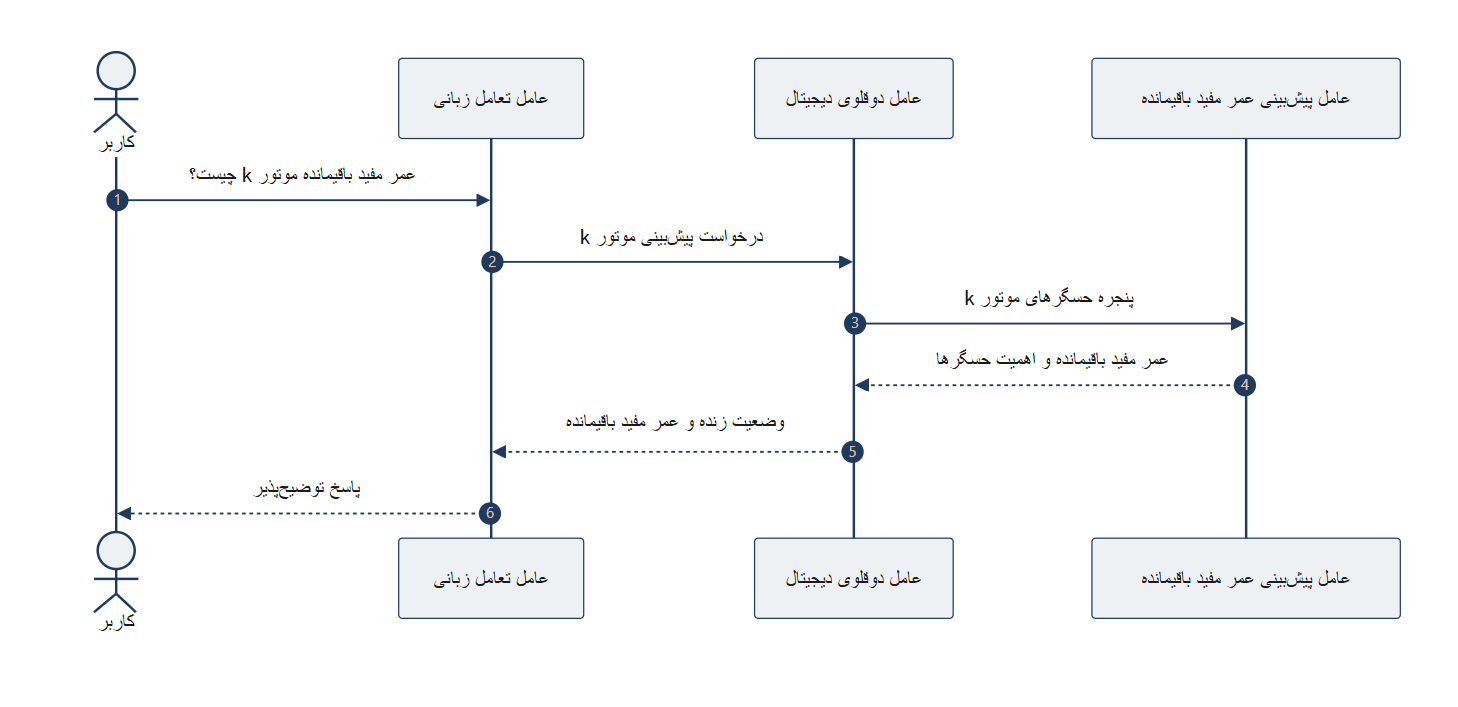
\includegraphics[width=1.1\textwidth]{images/arch_sequence4.png}
    \caption{
    	دیاگرام توالی تعامل برای پاسخ‌گویی به پرسش «عمر مفید باقیمانده موتور $k$ چیست؟»؛ درخواست از کاربر به عامل زبانی و سپس به عامل دوقلو و عامل پیش‌بینی منتقل می‌شود و نتیجه پس از به‌روزرسانی وضعیت دوقلو، به‌صورت پاسخ توضیح‌پذیر به کاربر بازمی‌گردد.}
    \label{fig:arch-sequence}
\end{figure}

مطابق شکل \ref{fig:arch-sequence}، نخست کاربر پرسش خود را از طریق رابط زبانی ارسال می‌کند. در گام دوم، عامل تعامل زبانی نیت کاربر را شناسایی کرده و شناسه $k$ را از عبارت ورودی استخراج می‌کند. در گام سوم، عامل دوقلوی دیجیتال درخواست مربوط به موتور $k$ را دریافت کرده و پنجره زمانی مورد نیاز برای پیش‌بینی را از لایه ادغام دریافت می‌کند؛ این پنجره شامل توالی آخرین اندازه‌گیری‌های حسگری مورد نیاز مدل \gls{RUL} است. در گام چهارم، عامل پیش‌بینی \gls{RUL} این توالی را به مدل تخصصی ارسال کرده و $\widehat{RUL}_k(t)$ را محاسبه می‌کند. در صورت استفاده از یک روش توضیح‌پذیر، اطلاعاتی مانند اهمیت نسبی حسگرها نیز در همین مرحله تولید می‌شود. در گام پنجم، نتیجه پیش‌بینی به عامل دوقلو بازگردانده شده و عامل دوقلو وضعیت زنده موتور را با مقدار جدید \gls{RUL} و سایر اطلاعات همراه به‌روزرسانی می‌کند. در گام ششم، عامل تعامل زبانی وضعیت ساختاریافته را دریافت کرده و پاسخ نهایی را تولید می‌کند؛ برای مثال، پاسخ می‌تواند شامل مقدار \gls{RUL}، وضعیت فعلی موتور، چرخه جاری، سطح هشدار و مهم‌ترین عوامل مؤثر بر پیش‌بینی باشد.

این توالی نشان می‌دهد که معماری پیشنهادی در واقع یک زنجیره ساده ``مدل‌های زبانی بزرگ $\rightarrow$ \gls{RUL}'' نیست، بلکه یک حلقه ``کاربر $\rightarrow$ مدل زبانی بزرگ $\rightarrow$ عامل دوقلوی دیجیتال $\rightarrow$ عامل \gls{RUL} $\rightarrow$ عامل دوقلوی دیجیتال $\rightarrow$ مدل زبانی بزرگ $\rightarrow$ کاربر'' است. این تمایز از منظر طراحی سامانه اهمیت دارد، زیرا دوقلو‌های دیجیتال در اینجا نقش حافظه وضعیت و واسط معنایی میان مدل‌های تخصصی و عامل‌های کاربردی را ایفا می‌کند. از سوی دیگر، مدل‌ زبانی بزرگ وظیفه تولید یا جعل وضعیت فیزیکی را ندارد، بلکه فقط بر اساس وضعیت بازیابی‌شده از دوقلوی دیجیتال، پاسخ و توضیح تولید می‌کند \cite{zhou2026dtai,fu2026genaidt}.

از دیدگاه نگهداری پیش‌بینانه، این معماری امکان گسترش فرایند پرسش و پاسخ ساده به فرآیندهای تصمیم‌گیری پیچیده‌تر را نیز فراهم می‌کند. برای مثال، پس از دریافت وضعیت موتور، یک عامل تشخیص می‌تواند علت احتمالی افت سلامت را بررسی کند، یک عامل برنامه‌ریزی می‌تواند زمان مناسب نگهداری را پیشنهاد دهد، یک عامل هزینه می‌تواند هزینه توقف و تعمیر را محاسبه کند و در نهایت عامل زبان طبیعی می‌تواند خروجی این عامل‌ها را برای کاربر ترکیب کند. چنین توسعه‌ای با روند اخیر حرکت از دوقلو‌های دیجیتال منفرد به دوقلو‌های دیجیتال چندعاملی و \glspl{Agentic Digital Twin}  سازگار است \cite{coulibaly2026madtdt}. در نتیجه، معماری حاضر می‌تواند به‌عنوان یک زیرساخت قابل توسعه برای حرکت از ``پیش‌بینی \gls{RUL}'' به \gls{Agentic Predictive Maintenance} مورد استفاده قرار گیرد.

بر این اساس، معماری پیشنهادی را می‌توان به‌صورت یک زنجیره لایه‌ای و در عین حال دوسویه تعریف کرد که در آن داده از موجودیت فیزیکی به سمت دانش و تصمیم حرکت می‌کند و فرمان یا درخواست در مسیر معکوس به سمت موجودیت بازمی‌گردد. این ساختار علاوه بر حفظ استقلال مدل‌های تخصصی، امکان افزودن مدل‌های زبانی بزرگ، عامل‌های جدید، روش‌های پیشرفته‌تر پیش‌بینی مانند \glspl{Transformer} و سازوکارهای تصمیم‌گیری چندعاملی را فراهم می‌سازد. از این منظر، ارزش اصلی معماری پیشنهادی در یک مدل یادگیری منفرد خلاصه نمی‌شود، بلکه در ایجاد یک چارچوب یکپارچه برای اتصال داده‌های حسگری، پیش‌بینی \gls{RUL}، وضعیت دوقلو‌های دیجیتال، استدلال زبانی و همکاری عامل‌ها است. چارچوبی که می‌تواند در مراحل بعدی پژوهش به سمت تصمیم‌گیری خودکار، برنامه‌ریزی نگهداری و حلقه بسته انسان--عامل--دوقلوی‌ دیجیتال توسعه یابد.

%------------------------------------------------------------------------

% -----------------------------------------------------------------------
\section{مجموعه داده \lr{CMAPSS} و آماده‌سازی داده}
\label{sec:dataset}

\subsection{معرفی و ساختار مجموعه داده}
\label{sec:dataset-intro}

برای ارزیابی تجربی معماری پیشنهادی، از مجموعه داده
\gls{CMAPSS} استفاده شده است. این مجموعه داده توسط مرکز پژوهشی
\lr{NASA Ames Research Center}
تولید شده و یکی از مجموعه داده‌های مرجع در پژوهش‌های مرتبط با
پیش‌بینی \gls{RUL} موتورهای جت به شمار
می‌رود \cite{NASA2007C-MAPSS}.
در این شبیه‌سازی، وضعیت موتور در چرخه‌های کاری متوالی ثبت می‌شود و
داده‌های حسگری حاصل از روند تخریب موتور، امکان توسعه و مقایسه
روش‌های مختلف پیش‌آگاهی و پیش‌بینی \gls{RUL} را فراهم می‌کند.

اهمیت \gls{CMAPSS} برای پژوهش حاضر از ماهیت چندمتغیره و زمانی داده‌ها
ناشی می‌شود. هر موتور به‌صورت یک دنباله زمانی مستقل مشاهده می‌شود و
مقادیر حسگرها در طول چرخه‌های متوالی تغییر می‌کنند. بنابراین، مسئله
تنها یک مسئله رگرسیون ایستا نیست، بلکه پیش‌بینی \gls{RUL} مستلزم
استخراج اطلاعات مرتبط با روند تغییرات وضعیت موتور، در طول زمان است.
به همین دلیل، این مجموعه داده از نخستین سنجه‌های مهم برای بررسی
روش‌های مبتنی بر شبکه‌های بازگشتی و همچنین روش‌های یادگیری عمیق در
پیش‌بینی \gls{RUL} بوده است \cite{heimes2008recurrent}.
همچنین، مطالعات بر روی مجموعه داده CMAPSS نشان داده‌اند که
تفاوت در شرایط عملیاتی، تعداد حالت‌های خرابی، نویز حسگرها و نحوه
پردازش داده می‌تواند تأثیر قابل‌توجهی بر مقایسه منصفانه مدل‌های
پیش‌بینی داشته باشد \cite{NASA2007C-MAPSS}.

مجموعه داده \gls{CMAPSS} از چهار زیرمجموعه
\lr{FD001} تا \lr{FD004} تشکیل شده است. این زیرمجموعه‌ها از نظر
تعداد شرایط عملیاتی و حالت‌های خرابی با یکدیگر تفاوت دارند. در
\lr{FD001} تنها یک شرایط عملیاتی و یک حالت خرابی در نظر گرفته شده
است؛ \lr{FD002} شامل شش شرایط عملیاتی و یک حالت خرابی است؛
\lr{FD003} شامل یک شرایط عملیاتی و دو حالت خرابی است؛ و
\lr{FD004} شامل شش شرایط عملیاتی و دو حالت خرابی است
\cite{NASA2007C-MAPSS}. از این منظر،
\lr{FD001} ساده‌ترین فرایند این مجموعه داده محسوب می‌شود و
\lr{FD004} پیچیده‌ترین ترکیب شرایط عملیاتی و حالت‌های خرابی را
ارائه می‌کند.

مشخصات چهار زیرمجموعه در جدول
\ref{tab:cmapss-subsets} ارائه شده است. در پژوهش حاضر، \lr{FD001}
به‌عنوان فرایند اصلی آزمایش انتخاب شده است. این انتخاب به معنای
برتری ذاتی \lr{FD001} نسبت به سایر زیرمجموعه‌ها نیست، بلکه با هدف
ایجاد یک سناریوی کنترل‌شده برای ارزیابی اولیه معماری انجام شده است.
از آنجا که در این زیرمجموعه تغییر شرایط عملیاتی و تنوع حالت خرابی
نسبت به \lr{FD002} و \lr{FD004} محدودتر است، می‌توان اثر معماری
پیشنهادی و مدل پیش‌بینی را با پیچیدگی کمتری بررسی کرد
\cite{NASA2007C-MAPSS}. ارزیابی زیرمجموعه‌های پیچیده‌تر می‌تواند
در ادامه به‌عنوان توسعه آزمایش‌ها انجام شود.

\begin{table}[ht]
	\centering
	\caption{مشخصات زیرمجموعه‌های مجموعه داده \lr{CMAPSS}}
	\label{tab:cmapss-subsets}
	\begin{tabular}{ccccc}
		\toprule
		\textbf{زیرمجموعه} &
		\textbf{شرایط عملیاتی} &
		\textbf{حالت خرابی} &
		\textbf{موتور آموزش} &
		\textbf{موتور آزمون} \\
		\midrule
		\lr{FD001} & ۱ & ۱ & ۱۰۰ & ۱۰۰ \\
		\lr{FD002} & ۶ & ۱ & ۲۶۰ & ۲۵۹ \\
		\lr{FD003} & ۱ & ۲ & ۱۰۰ & ۱۰۰ \\
		\lr{FD004} & ۶ & ۲ & ۲۴۸ & ۲۴۸ \\
		\bottomrule
	\end{tabular}
\end{table}

در سطح رکورد، داده خام \gls{CMAPSS} شامل ۲۶ ستون است که از شناسه
موتور، شماره چرخه کاری، سه متغیر تنظیم عملیاتی و ۲۱ متغیر حسگری
تشکیل می‌شود. شناسه موتور با \lr{unit\_number} مشخص شده و برای
تفکیک تاریخچه موتورهای مختلف به‌کار می‌رود. متغیر
\lr{time\_in\_cycles} نیز موقعیت مشاهده در چرخه عمر موتور را نشان
می‌دهد. سه متغیر تنظیم عملیاتی شرایط کاری شبیه‌سازی‌شده را توصیف
می‌کنند و ۲۱ حسگر اطلاعات مرتبط با وضعیت عملیاتی و سلامت موتور را
ثبت می‌کنند \cite{NASA2007C-MAPSS}.

از دیدگاه یادگیری ماشین، داده هر موتور را می‌توان به‌صورت یک سری
زمانی چندمتغیره نمایش داد. اگر $x_t \in \mathbb{R}^{d}$ بردار
ویژگی‌های موتور در چرخه $t$ باشد، تاریخچه موتور به‌صورت دنباله‌ای
از بردارهای
$\{\mathbf{x}_1,\mathbf{x}_2,\ldots,\mathbf{x}_T\}$
در نظر گرفته می‌شود. این ساختار امکان استفاده از مدل‌های توالی‌محور
مانند \gls{LSTM} را فراهم می‌کند؛ زیرا چنین مدل‌هایی می‌توانند
اطلاعات چند گام زمانی متوالی را در فرآیند برآورد \gls{RUL} لحاظ
کنند \cite{heimes2008recurrent}.

در آزمایش اصلی این پژوهش، فایل آموزش \lr{train\_FD001.txt}
شامل ۲۰۶۳۱ مشاهده مربوط به ۱۰۰ موتور است و تاریخچه هر موتور تا
چرخه خرابی در دسترس قرار دارد. فایل
\lr{test\_FD001.txt} نیز شامل ۱۳۰۹۶ مشاهده مربوط به ۱۰۰ موتور است؛
با این تفاوت که تاریخچه موتورهای آزمون پیش از خرابی متوقف شده است.
بنابراین، زمان واقعی خرابی موتورهای آزمون مستقیماً در فایل آزمون
مشاهده نمی‌شود و برای محاسبه مقدار واقعی \gls{RUL} باید از فایل
\lr{RUL\_FD001.txt} استفاده شود. این ساختار، مسئله آزمون را به
فرایندی نزدیک می‌کند که در آن وضعیت فعلی تجهیز مشاهده می‌شود اما
زمان خرابی آینده هنوز رخ نداده است \cite{NASA2007C-MAPSS}.

\subsection{تحلیل اکتشافی و انتخاب ویژگی}
\label{sec:eda}

پیش از تشکیل ورودی مدل، داده آموزشی از نظر تغییرپذیری ویژگی‌ها،
ارتباط با متغیر هدف و تغییرات مقادیر حسگر‌ها بررسی شد. هدف از
این مرحله کاهش ویژگی‌هایی است که یا فاقد اطلاعات تغییرپذیر هستند،
یا اطلاعات تکراری ارائه می‌کنند، یا در چارچوب آزمایش حاضر، ارزش
پیش‌بینی محدودی دارند. استفاده از چنین مرحله‌ای با رویه‌های رایج
در مطالعات \gls{CMAPSS} سازگار است. با این حال، مجموعه ویژگی نهایی باید
بر اساس داده و \gls{Protocol} همان پژوهش تعیین شود، زیرا انتخاب ویژگی در
مطالعات مختلف \gls{CMAPSS} یکسان نیست \cite{smith2025cmapsslinear,li2025attentiondt}.

در پژوهش حاضر، ابتدا ویژگی‌های فاقد تغییرپذیری مؤثر در داده
آموزشی شناسایی و حذف شدند. علاوه بر آن، همبستگی میان متغیرهای
حسگرها و \gls{RUL} بررسی شد تا متغیرهایی که در فرایند
\lr{FD001}
 اطلاعات محدودی ارائه می‌کنند مشخص شوند. در این مرحله،
ضریب همبستگی \lr{Pearson} به‌عنوان یک معیار توصیفی مورد استفاده
قرار گرفت. لازم به تأکید است که مقدار همبستگی به‌تنهایی مبنای
کافی برای حذف یک حسگر نیست؛ زیرا رابطه یک حسگر با \gls{RUL}
ممکن است غیرخطی یا وابسته به تاریخچه زمانی باشد. ازاین‌رو،
نتایج همبستگی در این پژوهش به‌عنوان ابزار تحلیل اکتشافی و نه یک
آزمون قطعی اهمیت ویژگی تفسیر شده‌اند.


پس از محاسبه برچسب \gls{RUL}، ضریب همبستگی \lr{Pearson} میان ویژگی‌های باقی‌مانده و متغیر هدف محاسبه شد. همان‌گونه که در شکل \ref{fig:corr-heatmap} مشاهده می‌شود، \gls{RUL} با \lr{time\_in\_cycles}، \lr{Ps30}، \lr{T50} و \lr{BPR} رابطه منفی نسبتاً قوی دارد؛ به این معنا که با افزایش چرخه‌های کاری و نزدیک شدن موتور به انتهای عمر، مقدار عمر مفید باقی‌مانده کاهش می‌یابد. در مقابل، ویژگی‌هایی نظیر \lr{phi}، \lr{W31} و \lr{W32} رابطه مثبت قابل‌توجهی با \gls{RUL} نشان می‌دهند. همچنین، دو متغیر \lr{setting\_1} و \lr{setting\_2} رابطه بسیار ضعیفی با متغیر هدف دارند و \lr{P15} نیز ارتباط محدودی نشان می‌دهد. نکته مهم دیگر، همبستگی بسیار بالای میان \lr{Nc} و \lr{NRc} با مقدار تقریبی $0.96$ است که نشان می‌دهد نگه‌داری هم‌زمان این دو متغیر می‌تواند اطلاعات تکراری وارد مدل کند. از این رو، انتخاب ویژگی در پژوهش حاضر صرفاً بر مبنای مقدار همبستگی با \gls{RUL} انجام نشده، بلکه ترکیبی از حذف ویژگی‌های ثابت، حذف ویژگی‌های کم‌اطلاع و کاهش هم‌خطی میان متغیرهای حسگری مورد توجه قرار گرفته است.


\begin{figure}[H]
	 \centering
	  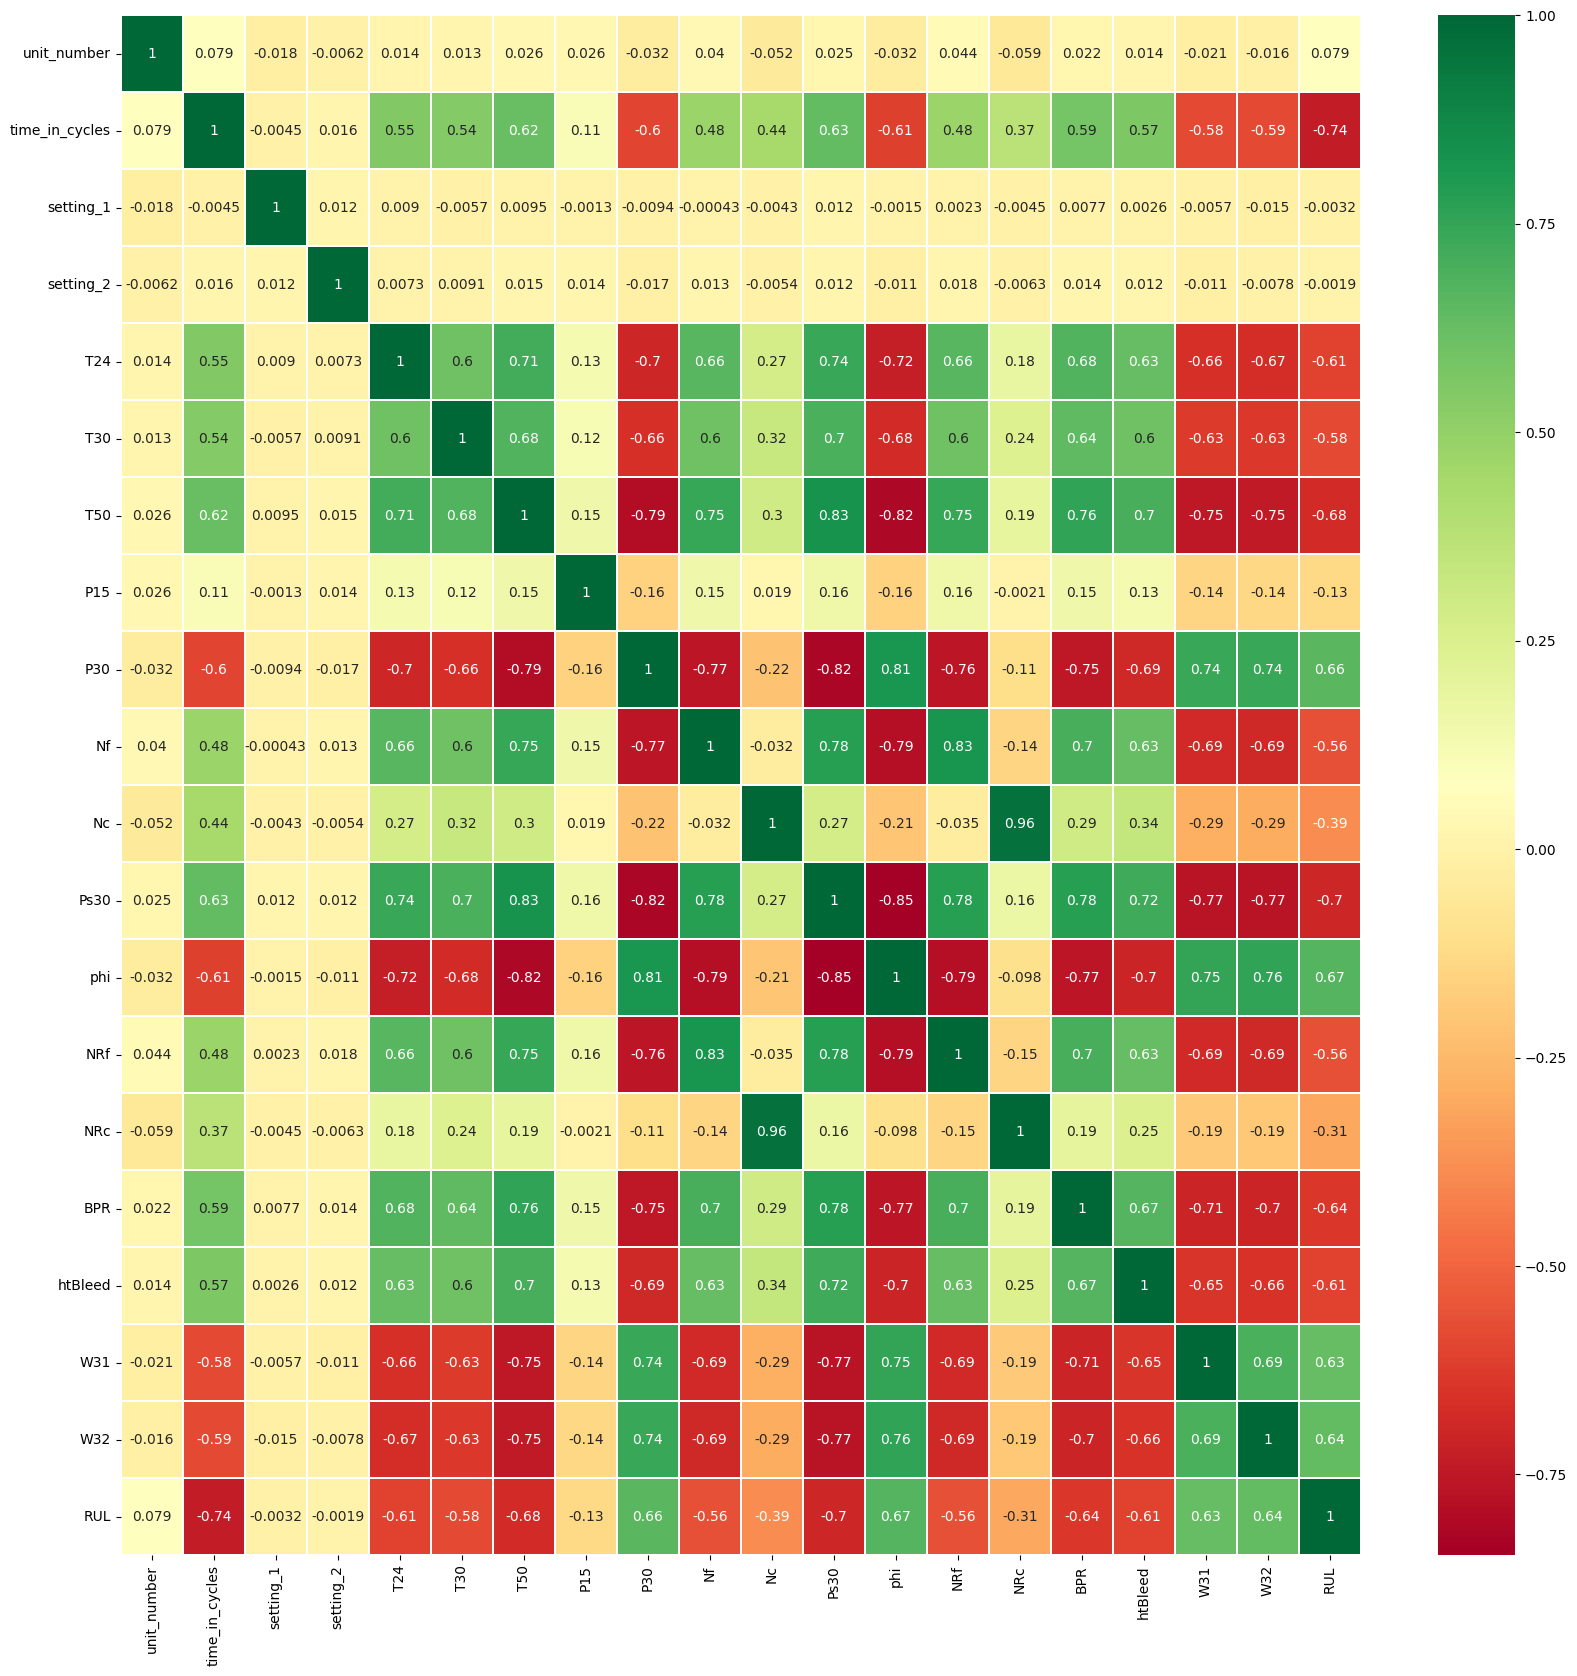
\includegraphics[width=0.98\textwidth] {images/cmapss_corr_heatmap.png}
	   \caption{نقشه همبستگی \lr{Pearson} ویژگی‌ها و برچسب عمر مفید باقیمانده در داده آموزشی \lr{FD001} پس از حذف ستون‌های ثابت} 
	   \label{fig:corr-heatmap} 
\end{figure}


بر اساس تحلیل انجام‌شده در پژوهش حاضر، ویژگی‌های
\lr{TRA}، \lr{T2}، \lr{P2}، \lr{epr}، \lr{farB}،
\lr{Nf\_dmd} و \lr{PCNfR\_dmd}
به دلیل داشتن مقدار ثابت و عدم ارائه اطلاعات مفید برای پیش‌بینی، از مجموعه ورودی حذف شدند.
همچنین \lr{setting\_1} و \lr{setting\_2} به دلیل اطلاعات محدود در
فرایند \lr{FD001} و \lr{P15} به دلیل ارزش پیش‌بینی پایین در
تحلیل حاضر کنار گذاشته شدند. افزون بر آن، به دلیل هم‌خطی شدید
میان \lr{Nc} و \lr{NRc}، تنها \lr{Nc} حفظ شد. چنین تصمیمی با
مشاهدات مطالعات پیشین درباره وجود ویژگی‌های کم‌اطلاع یا بسیار
هم‌بسته در داده‌های CMAPSS هم‌راستا است
\cite{smith2025cmapsslinear,li2025attentiondt}.

در نهایت، ۱۳ حسگر شامل
\lr{T24}، \lr{T30}، \lr{T50}، \lr{P30}، \lr{Nf}،
\lr{Nc}، \lr{Ps30}، \lr{phi}، \lr{NRf}، \lr{BPR}،
\lr{htBleed}، \lr{W31} و \lr{W32}
برای استفاده در مدل انتخاب شدند. علاوه بر این، شماره چرخه به‌صورت
هنجارشده با نام \lr{cycle\_norm} ایجاد شد تا موقعیت نسبی موتور در
طول عمر مشاهده‌شده آن به مدل ارائه شود. در جدول
 \ref{tab:feature-selection}
 مراحل انتخاب ویژگی به صورت خلاصه نشان داده می‌شود.


\begin{table}[ht]
	\centering
	\caption{فرایند انتخاب ویژگی در زیرمجموعه \lr{FD001}}
	\label{tab:feature-selection}
	\begin{tabular}{p{3.8cm}p{8.8cm}}
		\toprule
		\textbf{مرحله} & \textbf{ویژگی‌ها / تصمیم} \\
		\midrule
		حذف ویژگی‌های فاقد تغییرپذیری مؤثر &
		\lr{TRA}، \lr{T2}، \lr{P2}، \lr{epr}،
		\lr{farB}، \lr{Nf\_dmd} و \lr{PCNfR\_dmd} \\
		\addlinespace
		حذف ویژگی‌های کم‌اطلاع &
		\lr{setting\_1}، \lr{setting\_2} و \lr{P15} \\
		\addlinespace
		کاهش هم‌خطی &
		حذف \lr{NRc} و حفظ \lr{Nc} \\
		\addlinespace
		حسگرهای نهایی &
		\lr{T24}، \lr{T30}، \lr{T50}، \lr{P30}، \lr{Nf}،
		\lr{Nc}، \lr{Ps30}، \lr{phi}، \lr{NRf}،
		\lr{BPR}، \lr{htBleed}، \lr{W31} و \lr{W32} \\
		\bottomrule
	\end{tabular}
\end{table}

\subsection{پیش‌پردازش و تشکیل دنباله‌های زمانی}
\label{sec:preprocessing}

پس از پاک‌سازی و انتخاب ویژگی، داده‌ها برای استفاده در مدل
توالی‌محور به نمونه‌های زمانی با طول ثابت تبدیل شدند. نخستین
مرحله، محاسبه برچسب \gls{RUL} برای داده آموزشی است. از آنجا که
تاریخچه موتورهای آموزشی تا خرابی در دسترس است، اگر
$t_{\mathrm{end}}^{(i)}$ آخرین چرخه مشاهده‌شده برای موتور $i$
باشد، مقدار واقعی \gls{RUL} در چرخه $t$ از رابطه \ref{eq:rul-label} محاسبه می‌شود:

\begin{equation}
	\label{eq:rul-label}
	y^{(i)}(t)
	=
	t_{\mathrm{end}}^{(i)}-t.
\end{equation}

در نتیجه، مقدار \gls{RUL} در آخرین چرخه موتور برابر صفر است و
برای چرخه‌های قبل، متناسب با فاصله زمانی تا خرابی افزایش می‌یابد.
این تعریف با مسائل رایج 
\gls{RUL}
در داده‌های
\gls{run-to-failure}
 سازگار است \cite{NASA2007C-MAPSS,heimes2008recurrent}.


برای داده آزمون، دنباله هر موتور پیش از وقوع خرابی قطع شده است.
بنابراین، برخلاف داده آموزشی، لحظه خرابی در فایل آزمون مشاهده نمی‌شود.
فایل \lr{RUL\_FD001.txt} تنها مقدار \gls{RUL} را در آخرین چرخه
مشاهده‌شده هر موتور ارائه می‌دهد.
اگر $t_{\mathrm{last}}^{(i)}$ آخرین چرخه مشاهده‌شده موتور $i$
و $r_{\mathrm{file}}^{(i)}$ مقدار ثبت‌شده در این فایل باشد،
لحظه خرابی به‌صورت
$t_{\mathrm{fail}}^{(i)}=t_{\mathrm{last}}^{(i)}+r_{\mathrm{file}}^{(i)}$
بازسازی می‌شود.
سپس برچسب همه چرخه‌های همان موتور، مشابه رابطه~\eqref{eq:rul-label}،
از فاصله تا لحظه خرابی به‌دست می‌آید:

\begin{equation}
	\label{eq:rul-test}
	y^{(i)}(t)
	=
	t_{\mathrm{last}}^{(i)}
	+
	r_{\mathrm{file}}^{(i)}
	-
	t
	=
	t_{\mathrm{fail}}^{(i)}-t.
\end{equation}

در نتیجه، در آخرین چرخه مشاهده‌شده داریم
$y^{(i)}\bigl(t_{\mathrm{last}}^{(i)}\bigr)=r_{\mathrm{file}}^{(i)}$
و برچسب با مقدار مرجع ناسا یکی است.
ارزیابی کمی مدل نیز روی همین نقطه، یعنی آخرین پنجره زمانی هر موتور
آزمون، انجام می‌شود.

در مرحله بعد، ویژگی‌های حسگری منتخب با استفاده از تبدیل
\lr{Min-Max} به بازه $[0,1]$ منتقل شدند:

\begin{equation}
	\label{eq:normalization}
	x_{\mathrm{norm}}
	=
	\frac{x-x_{\min}}
	{x_{\max}-x_{\min}}.
\end{equation}

برای جلوگیری از نشت اطلاعات، پارامترهای $x_{\min}$ و $x_{\max}$
تنها از داده آموزشی محاسبه شدند و همان مقادیر برای تبدیل داده
آزمون مورد استفاده قرار گرفتند. بنابراین، هیچ اطلاعاتی از توزیع
داده آزمون برای تعیین پارامترهای پیش‌پردازش وارد مرحله آموزش
نمی‌شود.


در کنار ویژگی‌های حسگرها، متغیر \lr{cycle\_norm} نیز به‌عنوان
زمان نسبی هر موتور ایجاد شد و توالی داده را مشخص کرد. همچنین با استفاده از این متغیر می‌توان گذشت زمان را در دوقلوی دیجیتال شبیه‌سازی کرد. شناسه موتور و شماره چرخه خام برای مدیریت دنباله و نگهداری وضعیت موجودیت حفظ شدند. با این حال، همان‌گونه که در بخش انتخاب ویژگی توضیح داده شد،
شناسه موتور نباید بدون توجیه روش‌شناختی به‌عنوان یک متغیر فیزیکی
سلامت تفسیر شود.

پس از هنجارسازی، از یک پنجره لغزنده با طول
$w=50$ برای تبدیل داده‌های جدولی به نمونه‌های توالی استفاده شد.
اگر $\mathbf{x}_t$ بردار ویژگی موتور در چرخه $t$ باشد، ورودی مدل
در زمان $t$ به‌صورت 
\ref{eq:lstm-window}
 تعریف می‌شود.

\begin{equation}
	\label{eq:lstm-window}
	\mathbf{X}_{t-49:t}
	=
	[
	\mathbf{x}_{t-49},
	\mathbf{x}_{t-48},
	\ldots,
	\mathbf{x}_{t}
	].
\end{equation}

در نتیجه، هر نمونه ورودی دارای ۵۰ گام زمانی متوالی است. انتخاب
پنجره زمانی به مدل اجازه می‌دهد به‌جای اتکا به یک مشاهده منفرد،
الگوی تغییرات اخیر وضعیت موتور را در پیش‌بینی \gls{RUL} لحاظ کند.
این رویکرد با ماهیت مدل‌های بازگشتی و مطالعات استفاده از LSTM برای
پیش‌بینی \gls{RUL} سازگار است \cite{heimes2008recurrent}.

برچسب هر پنجره برابر با مقدار \gls{RUL} در آخرین چرخه همان پنجره
در نظر گرفته می‌شود. بنابراین، اگر پنجره مربوط به چرخه‌های
$t-49$ تا $t$ باشد، هدف آن $y(t)$ خواهد بود. در نتیجه، هر نمونه
آموزشی اطلاعات تاریخی لازم برای تخمین عمر باقی‌مانده در انتهای
پنجره را در اختیار مدل قرار می‌دهد.

در نهایت، تفکیک آموزش و آزمون در سطح موتور حفظ شد و هیچ تقسیم
تصادفی از پنجره‌های زمانی انجام نشد. این تصمیم از اهمیت
روش‌شناختی بالایی برخوردار است؛ زیرا پنجره‌های متوالی یک موتور
دارای هم‌پوشانی زمانی زیادی هستند و تقسیم تصادفی آن‌ها میان
آموزش و آزمون می‌تواند موجب انتقال اطلاعات بسیار مشابه میان دو
مجموعه و در نتیجه برآورد خوش‌بینانه عملکرد مدل شود. حفظ \gls{Protocol}
اصلی \gls{CMAPSS} و تفکیک موتورهای آموزش و آزمون، امکان مقایسه منصفانه‌تر
با مطالعات پیشین را فراهم می‌کند \cite{NASA2007C-MAPSS}.


% =======================================================================

% انطباق معماری پیشنهادی بر مسئله CMAPSS

% =======================================================================

\section{انطباق معماری پیشنهادی بر مسئله \lr{CMAPSS}}
\label{sec:arch-cmapss}

پس از آماده‌سازی داده، مرحله بعدی پژوهش به نگاشت معماری پیشنهادی
بر مسئله مشخص پیش‌بینی \gls{RUL} اختصاص می‌یابد. هدف این نگاشت،
تبدیل معماری مفهومی معرفی‌شده در فصل‌های پیشین به یک نمونه قابل
پیاده‌سازی و ارزیابی است؛ به‌گونه‌ای که مشخص شود داده از لحظه ورود
به سامانه تا تولید پیش‌بینی و ارائه آن به کاربر چگونه در میان
اجزای مختلف معماری جریان پیدا می‌کند.

در این پژوهش، داده‌های \gls{CMAPSS} به‌عنوان داده شبیه‌سازی‌شده
از رفتار موتورهای جت در طول چرخه عمر در نظر گرفته می‌شوند و نه
به‌عنوان داده حاصل از یک سامانه فیزیکی برخط. بنابراین، نیاز است تا لایه‌های مربوط به معماری به اجزای این مسئله نگاشت شود. \cite{qi2021enabling,tao2018digital}.

\subsection{نگاشت لایه‌ها به اجزای مسئله}
\label{sec:layer-mapping}

در لایه موجودیت، هر موتور موجود در زیرمجموعه \lr{FD001} به‌عنوان
یک موجودیت مستقل در نظر گرفته می‌شود. شناسه \lr{unit\_number}
برای شناسایی این موجودیت و ویژگی‌های آن استفاده
می‌شود. تاریخچه چرخه‌های کاری و داده‌های حسگرهای هر موتور نیز وضعیت آن موجودیت را تشکیل می‌دهد.

لایه جمع‌آوری داده مسئول دریافت مشاهدات چرخه‌ای از مجموعه داده
است. در پیاده‌سازی آزمایشگاهی، داده‌ها از فایل‌های
\gls{CMAPSS} خوانده می‌شوند و به‌صورت ترتیبی در اختیار اجزای
بعدی سامانه قرار می‌گیرند. بنابراین، اگرچه منشأ داده یک فایل
آموزشی یا آزمونی است، جریان داده در معماری به‌گونه‌ای سازمان‌دهی
می‌شود که دریافت متوالی داده‌های حسگری یک سامانه پایش را بازنمایی
کند.

لایه ادغام مسئول تبدیل داده خام به یک نمایش استاندارد برای اجزای
تحلیلی سامانه است. این لایه شامل انتخاب ویژگی، هنجارسازی و تشکیل
دنباله زمانی است. در آزمایش حاضر، ۱۳ حسگر منتخب پس از
پیش‌پردازش در پنجره‌های زمانی ۵۰ چرخه‌ای سازمان‌دهی می‌شوند.
خروجی این لایه، بنابراین، یک رکورد منفرد حسگری نیست، بلکه یک
نمایش زمانی ساختاریافته است که عامل پیش‌بینی می‌تواند آن را
پردازش کند.

این تفکیک مسئولیت اهمیت معماری دارد؛ زیرا عامل پیش‌بینی نباید
هم‌زمان مسئول مدیریت فایل خام، انتخاب ویژگی و تشکیل پنجره زمانی
باشد. جدا کردن این وظایف موجب کاهش وابستگی میان اجزای سامانه و
امکان جایگزینی مستقل عامل پیش‌بینی یا عامل پردازش داده می‌شود. چنین
نگاهی با رویکردهای سرویس‌محور در معماری دوقلوهای دیجیتال نیز
هم‌خوانی دارد \cite{qi2021enabling,tao2018digital}.

\begin{table}[ht]
	\centering
	\caption{نگاشت لایه‌های معماری پیشنهادی به اجزای پیاده‌سازی در مسئله \gls{CMAPSS}}
	\label{tab:layer-mapping}

	\begin{tabular}{p{3.6cm}p{4.8cm}p{5.2cm}}
		\toprule
		\textbf{لایه} & \textbf{نقش معماری} & \textbf{مصداق در آزمایش} \\
		\midrule
		\gls{EmtityLayer}
		&
		نمایندگی موجودیت
		&
		موتورهای شبیه‌سازی‌شده \lr{FD001}
		\\
		\addlinespace
		\gls{DataCollectionLayer}
		&
		دریافت داده چرخه‌ای
		&
		خواندن ترتیبی مشاهدات \gls{CMAPSS}
		\\
		\addlinespace
		\gls{IntegrationLayer}
		&
		استانداردسازی و ساخت توالی
		&
		انتخاب ویژگی، \lr{Min-Max} و پنجره $w=50$
		\\
		\addlinespace
		\gls{DigitalTwinAgentsLayer}
		&
		نگهداری وضعیت دیجیتال
		&
		وضعیت جاری هر موتور در سامانه
		\\
		\addlinespace
		\gls{ApplicationAgentsLayer}
		&
		ارائه خدمات تحلیلی و تعاملی
		&
		عامل پیش‌بینی، پایش، تعامل زبانی و \gls{Dashboard}
		\\
		\bottomrule

	\end{tabular}

\end{table}

در لایه عامل‌های دوقلوی دیجیتال، برای هر موتور یک وضعیت دیجیتال
قابل به‌روزرسانی نگهداری می‌شود. این وضعیت می‌تواند شامل شناسه
موتور، آخرین چرخه مشاهده‌شده، آخرین پنجره حسگری، آخرین مقدار
پیش‌بینی‌شده \gls{RUL} و وضعیت پایش باشد. بنابراین، دوقلو در این
پژوهش صرفاً یک رکورد ثابت از موتور نیست، بلکه یک ساختار نرم‌افزاری
برای نگهداری و به‌روزرسانی وضعیت موجودیت است.

این برداشت با مفهوم دوقلوی دیجیتال به‌عنوان پیوند میان موجودیت
فیزیکی و نمایش دیجیتال آن سازگار است؛ با این تفاوت که در آزمایش
حاضر، موجودیت فیزیکی مستقیماً به یک حسگر برخط متصل نیست و وضعیت
آن از داده شبیه‌سازی‌شده \gls{CMAPSS} دریافت می‌شود
\cite{tao2018digital,qi2021enabling}. بنابراین، عبارت «دوقلوی دیجیتال
آزمایشی» برای توصیف دقیق‌تر پیاده‌سازی حاضر مناسب‌تر از ادعای
وجود یک دوقلوی دیجیتال کامل در محیط واقعی است. اما با این حال، معماری پیشنهادی دوقلوی دیجیتال و چگونگی پیاده‌سازی‌ها در این آزمایش کاملا قابل تعمیم به یک دوقلوی دیجیتال در محیط واقعی است.

در لایه عامل‌های کاربردی، خدمات تخصصی سامانه از یکدیگر جدا
می‌شوند. عامل پیش‌بینی، مسئول اجرای مدل \gls{LSTM} و تولید
$\widehat{RUL}$ است. عامل پایش، خروجی مدل را دریافت کرده و بر اساس
قواعد تعیین‌شده، وضعیت موتور را ارزیابی می‌کند. عامل تعامل زبانی،
رابط میان کاربر و خدمات سامانه را فراهم می‌کند و عامل 
\gls{Dashboard}،
وظیفه نمایش وضعیت موتورها را بر عهده دارد.

این تفکیک با منطق سامانه‌های چندعاملی سازگار است؛ زیرا هر عامل
مسئولیت مشخصی دارد و هماهنگی میان آن‌ها از طریق وضعیت و پیام‌های
ساختاریافته انجام می‌شود. مطالعات جدید درباره ترکیب سامانه‌های
چندعاملی و دوقلوهای دیجیتال نیز بر همین موضوع، یعنی تفکیک نقش‌ها،
هماهنگی عامل‌ها و استفاده از دوقلوی دیجیتال به‌عنوان نمایش وضعیت سامانه،
تأکید دارند \cite{lopez2024madtwin,pretel2022masdt}.

\subsection{عامل پیش‌بینی و اتصال آن به جریان داده}
\label{sec:cmapss-prediction-agent}

در معماری پیشنهادی، پیش‌بینی عددی \gls{RUL} به یک عامل تخصصی
واگذار شده است. این عامل مدل \gls{LSTM} به همراه سازوکار توجه را
به‌عنوان یک خدمت تحلیلی در اختیار سایر اجزای سامانه قرار می‌دهد.
ورودی عامل پیش‌بینی، آخرین پنجره زمانی تولیدشده توسط لایه ادغام
است و خروجی اصلی آن مقدار عددی $\widehat{RUL}$ است.

استفاده از \gls{LSTM} در این بخش بر ماهیت زمانی مسئله استوار است.
\lr{Heimes} نشان داد که شبکه‌های بازگشتی می‌توانند برای مدل‌سازی
توالی‌های حاصل از روند تخریب مورد استفاده قرار گیرند
\cite{heimes2008recurrent}.
 مطالعات بعدی نیز نشان داده‌اند که LSTM با
حفظ اطلاعات زمانی طولانی‌تر می‌تواند برای تخمین \gls{RUL} از
داده‌های حسگری چندمتغیره مناسب باشد \cite{heimes2008recurrent}.
ازاین‌رو، در معماری حاضر مدل یادگیری عمیق وظیفه‌ای تخصصی و
قابل ارزیابی را بر عهده دارد و خروجی آن به‌صورت یک سرویس در
اختیار سایر عامل‌ها قرار می‌گیرد.

نکته مهم در طراحی حاضر، جداسازی مسیر استنتاج عددی از مسیر
تعامل زبانی است. مدل زبانی مستقیماً مسئول تولید مقدار عددی
\gls{RUL} نیست؛ بلکه مقدار پیش‌بینی‌شده توسط عامل تخصصی را
دریافت می‌کند و در صورت نیاز آن را برای کاربر تفسیر یا توضیح
می‌دهد. بنابراین، صحت مقدار \gls{RUL} را می‌توان مستقل از کیفیت
تولید متن ارزیابی کرد.

در سطح تابع هدف نیز هزینه خطا به‌صورت متقارن در نظر گرفته
نمی‌شود. در مسئله پیش‌بینی \gls{RUL}، کم‌برآورد و بیش‌برآورد عمر
مفید باقیمانده الزاماً پیامدهای یکسانی ندارند؛ به‌ویژه، بیش‌برآورد
\gls{RUL} می‌تواند موجب تأخیر در تصمیم‌گیری برای انجام عملیات
نگهداری و در نتیجه افزایش احتمال ادامه بهره‌برداری از تجهیز در
شرایط نزدیک به خرابی شود. ازاین‌رو، در پژوهش‌های جدید پیش‌بینی
\gls{RUL} بر روی مجموعه داده \gls{CMAPSS} نیز توجه به جهت خطای
پیش‌بینی و استفاده از معیارها یا توابع هزینه نامتقارن مورد توجه
قرار گرفته است \cite{he2025bilstmgru,zhang2026multistatistic,dong2026bidirectional}. 
در این رویکردها، هدف صرفاً کاهش خطای عددی پیش‌بینی نیست، بلکه
جلوگیری از خطاهای بیش‌برآوردی که می‌توانند هشدار دیرهنگام ایجاد
کنند نیز اهمیت دارد. به همین دلیل، در پژوهش حاضر نیز تابع هدف
به‌گونه‌ای انتخاب شده است که نسبت به جهت خطای پیش‌بینی حساس باشد
و مدل را به سمت برآورد محافظه‌کارانه‌تر \gls{RUL} هدایت کند. در پژوهش حاضر، برای ایجاد
این سوگیری از تابع زیان \lr{Pinball} با
$\tau=0.125$ استفاده شده است.

در سطح تابع هدف، هزینه خطای پیش‌بینی به‌صورت نامتقارن
تعریف شده است تا تفاوت میان پیامدهای عملیاتی کم‌برآورد و
بیش‌برآورد \gls{RUL} در فرایند آموزش مدل منعکس شود. در این
چارچوب، فرض بر آن است که بیش‌برآورد عمر مفید باقیمانده، یعنی
پیش‌بینی مقداری بزرگ‌تر از عمر واقعی تجهیز، می‌تواند موجب
به‌تعویق‌افتادن تصمیم نگهداری و افزایش ریسک بهره‌برداری تا
نزدیکی خرابی شود. به همین دلیل، در کاربردهای پیش‌بینی مبتنی بر
خطر، استفاده از توابع زیان نامتقارن و به‌ویژه زیان
\lr{Pinball}
 امکان کنترل جهت‌دار خطای پیش‌بینی را فراهم
می‌کند. این تابع با تعریف هزینه متفاوت برای خطاهای مثبت و منفی،
به مدل اجازه می‌دهد به‌جای تمرکز صرف بر کمینه‌سازی خطای متوسط،
به سمت خطای مورد نظر نسبت به متغیر هدف متمایل شود
\cite{Robinson2026riskaware}.

اگر $e=y-\hat{y}$ خطای پیش‌بینی تعریف شود که در آن $y$ مقدار
\gls{RUL}
و $\hat{y}$ مقدار پیش‌بینی شده باشد، تابع زیان \lr{Pinball}
برای
\gls{Quantile}
 $\tau$ به‌صورت زیر بیان می‌شود:

\begin{equation}
	\label{eq:pinball-loss}
	L_{\tau}(e)
	=
	\begin{cases}
		\tau e, & e \geq 0,\\
		(\tau-1)e, & e < 0.
	\end{cases}
\end{equation}

در این تعریف، 
$e>0$
 متناظر با کم‌برآوردی، یعنی
$\hat{y}<y$،
 و 
 $e<0$ 
 متناظر با بیش‌برآوردی، یعنی
$\hat{y}>y$، است. بنابراین، برای خطای کم‌برآورد ضریب $\tau$ و
برای خطای بیش‌برآورد ضریب $1-\tau$ در نظر گرفته می‌شود. در
پژوهش حاضر با انتخاب $\tau=0.125$، تابع هدف به کم‌برآورد و
بیش‌برآورد وزن یکسانی نمی‌دهد؛ به‌طوری‌که شیب تابع زیان در سمت
کم‌برآورد برابر $0.125$ و در سمت بیش‌برآورد برابر $0.875$ است.
در نتیجه، برای خطاهایی با قدرمطلق یکسان، هزینه بیش‌برآورد
هفت برابر هزینه کم‌برآورد خواهد بود. این نامتقارن‌سازی باعث
می‌شود مدل در فرایند بهینه‌سازی نسبت به بیش‌برآورد \gls{RUL}
حساس‌تر شود و در صورت وجود عدم‌قطعیت در داده، به سمت برآورد
محافظه‌کارانه‌تر متمایل گردد. در اینجا، محافظه‌کارانه بودن به
معنای افزایش احتمال کم‌برآورد کنترل‌شده عمر واقعی است و نه
الزاماً افزایش دقت مطلق پیش‌بینی. از این رو، اثر انتخاب
$\tau=0.125$
 باید در کنار معیارهای عمومی خطا و معیارهای حساس
به جهت خطا ارزیابی شود تا مشخص شود که کاهش ریسک بیش‌برآورد با
حفظ سطح قابل قبول دقت پیش‌بینی همراه بوده است.

\subsection{فرایند تعامل چندعاملی و دوقلوی دیجیتال}
\label{sec:e2e-scenario}

برای بررسی انسجام معماری، جریان سرتاسری سامانه از دریافت داده تا
ارائه پاسخ به کاربر به‌صورت یک سناریوی چندعاملی تعریف شده است.
در این فرایند، مشاهده جدید موتور ابتدا وارد لایه جمع‌آوری می‌شود.
پس از انجام پیش‌پردازش و تشکیل پنجره زمانی، وضعیت دوقلوی دیجیتال
موتور مربوطه به‌روزرسانی می‌شود. سپس عامل پیش‌بینی آخرین وضعیت
قابل استفاده را دریافت کرده و مقدار $\widehat{RUL}$ را محاسبه
می‌کند.

خروجی عامل پیش‌بینی در ادامه به عامل پایش منتقل می‌شود. عامل
پایش می‌تواند مقدار پیش‌بینی‌شده را با آستانه‌های عملیاتی تعریف‌شده
مقایسه کرده و وضعیت موتور را به‌عنوان وضعیت عادی، هشدار یا بحرانی
طبقه‌بندی کند. نتیجه این مرحله در وضعیت دوقلو ثبت می‌شود و برای
عامل تعامل زبانی و \gls{Dashboard} قابل دسترسی خواهد بود.

در صورت دریافت پرسش کاربر، عامل تعامل زبانی ابتدا درخواست را به
یک عملیات ساختاریافته تبدیل می‌کند. برای مثال، در پرسش
«\gls{RUL} موتور $k$ چقدر است؟»، شناسه موتور و نوع عملیات از
درخواست استخراج می‌شود. سپس عامل مربوطه وضعیت موتور $k$ را از
دوقلو دریافت کرده و در صورت نیاز عامل پیش‌بینی را فراخوانی
می‌کند. نتیجه عددی پس از بازگشت به عامل تعامل زبانی، به همراه
اطلاعات وضعیت موجود، برای تولید پاسخ طبیعی مورد استفاده قرار
می‌گیرد.

% =======================================================================
% روش ارزیابی طراحی‌شده

% =======================================================================
\section{روش ارزیابی طراحی‌شده}
\label{sec:eval-design}

روش ارزیابی پژوهش حاضر با هدف بررسی هم‌زمان عملکرد مدل پیش‌بینی
و قابلیت‌های معماری پیشنهادی طراحی شده است. از آنجا که هدف پژوهش
تنها توسعه یک مدل رگرسیون برای تخمین \gls{RUL} نیست، ارزیابی در
دو سطح اصلی انجام می‌شود. سطح نخست، ارزیابی مدل تخصصی پیش‌بینی از
نظر دقت و جهت خطا و سطح دوم، ارزیابی سامانه از نظر عملکرد جریان
چندعاملی و تعامل با کاربر است.

این تفکیک اهمیت دارد، زیرا بهبود عملکرد یک مدل \gls{LSTM}
لزوماً به معنای بهبود عملکرد کل سامانه نیست. برای مثال، ممکن است
مدل پیش‌بینی مقدار مناسبی برای \gls{RUL} تولید کند، اما عامل
تعامل نتواند درخواست کاربر را به سرویس مناسب هدایت کند. از سوی
دیگر، پاسخ زبانی مناسب نیز نمی‌تواند ضعف مدل عددی را جبران کند.
بنابراین، نتایج این دو سطح به‌صورت مستقل گزارش و سپس در سطح
معماری تفسیر می‌شوند.

\subsection{معیارهای کمی پیش‌بینی}
\label{sec:prediction-metrics}

برای سنجش دقت عددی مدل، معیارهای \lr{MAE} و \lr{RMSE} به‌عنوان
معیارهای اصلی و $R^2$ به‌عنوان معیار تکمیلی محاسبه می‌شوند.
معیار \lr{MAE} که در رابطه \ref{eq:mae} نشان داده شده، میانگین قدرمطلق خطا را اندازه‌گیری می‌کند.

\begin{equation}
	\label{eq:mae}
	\mathrm{MAE}
	=
	\frac{1}{N}
	\sum_{i=1}^{N}
	\left|
	\hat{y}_i-y_i
	\right|.
\end{equation}

در این رابطه، $N$ تعداد نمونه‌های ارزیابی، $y_i$ مقدار واقعی
\gls{RUL} و $\hat{y}_i$ مقدار پیش‌بینی‌شده است. مقدار کمتر
\lr{MAE} نشان‌دهنده فاصله متوسط کمتر میان پیش‌بینی و مقدار واقعی
است.

معیار \lr{RMSE} با مجازات بیشتر خطاهای بزرگ تعریف می‌شود. رابطه \ref{eq:rmse} این معیار را نشان می‌دهد.

\begin{equation}
	\label{eq:rmse}
	\mathrm{RMSE}
	=
	\sqrt{
		\frac{1}{N}
		\sum_{i=1}^{N}
		(\hat{y}_i-y_i)^2
	}.
\end{equation}

به دلیل وجود توان دوم، یک خطای بزرگ تأثیر بیشتری بر مقدار
\lr{RMSE}
 دارد. بنابراین، استفاده هم‌زمان از 
 \lr{MAE} و
\lr{RMSE} 
امکان تفکیک خطای متوسط از حساسیت مدل به خطاهای بزرگ را
فراهم می‌کند.

برای ارزیابی تکمیلی، ضریب تعیین $R^2$ که در رابطه 
\ref{eq:r2}
آمده است، نیز محاسبه می‌شود:

\begin{equation}
	\label{eq:r2}
	R^2
	=
	1-
	\frac{
		\sum_{i=1}^{N}
		(\hat{y}_i-y_i)^2
	}{
		\sum_{i=1}^{N}
		(y_i-\bar{y})^2
	}.
\end{equation}

در این رابطه، $\bar{y}$ میانگین مقادیر واقعی \gls{RUL} است.
مقدار بالاتر $R^2$ در حالت معمول نشان‌دهنده توانایی بیشتر مدل در
توضیح تغییرپذیری متغیر هدف است. با این حال، در مسئله
\gls{RUL}،
 $R^2$
  به‌تنهایی برای ارزیابی مناسب نیست و در این
پژوهش در کنار \lr{MAE} و \lr{RMSE} گزارش می‌شود.

\subsection{امتیاز ناسا و ارزیابی جهت خطا}
\label{sec:nasa-score}

با توجه به نامتقارن بودن هزینه خطا در مسئله نگهداری پیش‌بینانه،
ارزیابی مدل تنها بر اساس معیارهای متقارن کافی نیست. دو مدل ممکن
است \lr{RMSE} مشابهی داشته باشند، اما یکی عمدتاً \gls{RUL} را
بیش‌برآورد و دیگری عمدتاً کم‌برآورد کند. این دو رفتار از دیدگاه
نگهداری پیش‌بینانه پیامد یکسانی ندارند.

از این رو، امتیاز متداول مورد استفاده در ارزیابی CMAPSS نیز
گزارش می‌شود. اگر

\begin{equation}
	d_i=\hat{y}_i-y_i,
\end{equation}

باشد، تابع امتیاز هر نمونه به‌صورت زیر تعریف می‌شود:

\begin{equation}
	\label{eq:nasa-score}
	s_i
	=
	\begin{cases}
		\exp\left(\dfrac{d_i}{10}\right)-1,
		& d_i \geq 0,\\[8pt]
		\exp\left(\dfrac{-d_i}{13}\right)-1,
		& d_i < 0.
	\end{cases}
\end{equation}

امتیاز کل برابر است با:

\begin{equation}
	\label{eq:nasa-score-total}
	S
	=
	\sum_{i=1}^{N}s_i.
\end{equation}

در این تعریف، $d_i>0$ نشان‌دهنده بیش‌برآورد \gls{RUL} و
$d_i<0$ نشان‌دهنده کم‌برآورد است. بنابراین، خطای بیش‌برآورد با
پارامتر ۱۰ و خطای کم‌برآورد با پارامتر ۱۳ وارد تابع نمایی
می‌شوند. به دلیل شکل تابع نمایی، امتیاز برای خطاهای بزرگ به‌سرعت
افزایش می‌یابد و مقدار کمتر امتیاز نشان‌دهنده عملکرد بهتر است
\cite{NASA2007C-MAPSS}.

این معیار از این جهت برای پژوهش حاضر اهمیت دارد که هدف تابع
زیان انتخاب‌شده نیز کاهش تمایل مدل به بیش‌برآورد است. با وجود
این، امتیاز ناسا نباید با تابع زیان \lr{Pinball} یکسان تلقی شود؛
اولی یک معیار ارزیابی پس از آموزش است، در حالی که دومی مستقیماً
در فرآیند آموزش مدل استفاده می‌شود.

برای سنجش مستقیم جهت خطا، نسبت کم‌برآورد نیز محاسبه می‌شود:

\begin{equation}
	\label{eq:bias-ratio}
	r_{\mathrm{under}}
	=
	\frac{
		\left|
		\left\{
		i:\hat{y}_i<y_i
		\right\}
		\right|
	}{
		N
	}.
\end{equation}

مقدار بالاتر $r_{\mathrm{under}}$ نشان‌دهنده آن است که سهم بیشتری
از پیش‌بینی‌ها در سمت کم‌برآورد قرار گرفته‌اند. در این پژوهش،
این شاخص به‌تنهایی معیار «خوب بودن» مدل تلقی نمی‌شود؛ زیرا
افزایش بیش از حد کم‌برآورد نیز می‌تواند باعث کاهش دقت و افزایش
هزینه نگهداری غیرضروری شود. هدف، بررسی وجود یک سوگیری کنترل‌شده
به سمت کم‌برآورد در کنار حفظ دقت قابل قبول است.

بنابراین، اثر تابع زیان نامتقارن با ترکیب چهار شاخص
\lr{MAE}، \lr{RMSE}، امتیاز ناسا و $r_{\mathrm{under}}$ تحلیل
خواهد شد. این ترکیب امکان بررسی هم‌زمان مقدار خطا، حساسیت به
خطاهای بزرگ، هزینه نامتقارن و جهت خطا را فراهم می‌کند.

\subsection{ارزیابی عملکرد سامانه چندعاملی}
\label{sec:multiagent-metrics}

ارزیابی معماری پیشنهادی در سطح سامانه نیز به‌صورت مستقل از مدل
پیش‌بینی انجام می‌شود. در این سطح، سه دسته شاخص در نظر گرفته
می‌شود: زمان پاسخ، صحت مسیریابی درخواست و کیفیت پاسخ توضیحی.

شاخص نخست، زمان پاسخ سامانه است. این معیار فاصله زمانی میان
دریافت یک درخواست یا مشاهده جدید و تولید پاسخ مربوطه را اندازه‌گیری
می‌کند. در صورت استفاده از پردازش برخط، میانگین، میانه و صدک‌های
بالای زمان پاسخ می‌توانند گزارش شوند تا علاوه بر رفتار متوسط،
تأخیرهای غیرمعمول نیز مشخص شوند.

شاخص دوم، صحت اجرای درخواست است. در این ارزیابی، مجموعه‌ای از
درخواست‌های از پیش تعریف‌شده به سامانه ارائه می‌شود و بررسی
می‌شود که آیا عامل تعامل زبانی توانسته است نوع عملیات و موجودیت
مورد نظر را به‌درستی تشخیص داده و درخواست را به عامل مناسب
هدایت کند یا خیر. این معیار برای معماری حاضر اهمیت ویژه‌ای دارد،
زیرا عامل زبانی مسئول تولید مستقیم مقدار عددی \gls{RUL} نیست؛
بلکه باید درخواست زبان طبیعی را به عملیات ساختاریافته تبدیل کند.

شاخص سوم، کیفیت پاسخ توضیحی است. برای جلوگیری از ارزیابی صرفاً
زبانی، این شاخص باید بر مؤلفه‌های قابل بررسی متمرکز شود. از جمله
این مؤلفه‌ها می‌توان به صحت مقدار گزارش‌شده \gls{RUL}، انطباق
توضیح با وضعیت ثبت‌شده موتور، عدم افزودن اطلاعاتی که در وضعیت
سامانه وجود ندارد و خوانایی پاسخ اشاره کرد. بنابراین، ارزیابی
کیفیت توضیح باید میان «روان بودن متن» و «صحت محتوای فنی» تمایز
قائل شود.

در این چارچوب، عامل زبانی به‌عنوان جایگزین مدل پیش‌بینی ارزیابی
نمی‌شود. صحت پیش‌بینی عددی با معیارهای \lr{MAE}، \lr{RMSE}،
$R^2$ و امتیاز ناسا سنجیده می‌شود، در حالی که عملکرد عامل زبانی
در سطح تعامل و تبدیل اطلاعات ساختاریافته به پاسخ طبیعی ارزیابی
می‌شود. این تفکیک، امکان تعیین منشأ خطا را نیز فراهم می‌کند؛
برای مثال، می‌توان مشخص کرد که یک پاسخ نادرست ناشی از خطای
مدل پیش‌بینی \gls{RUL} بوده یا از مسیریابی نادرست عامل تعامل ناشی شده است.

\subsection{خطوط مبنا و مقایسه تجربی}
\label{sec:baselines}

برای تعیین جایگاه مدل پیشنهادی، عملکرد آن باید در شرایط یکسان با
چند خط مبنای معتبر مقایسه شود. این خطوط مبنا ترجیحاً از میان
مدل‌هایی انتخاب می‌شوند که \gls{Protocol} آزمایشی آن‌ها، زیرمجموعه
\gls{CMAPSS} و نحوه محاسبه \gls{RUL} به اندازه کافی مشخص باشد.
مطالعاتی که از LSTM، شبکه‌های توجه و مدل‌های رگرسیونی برای
CMAPSS استفاده کرده‌اند می‌توانند مبنای این مقایسه قرار گیرند
\cite{heimes2008recurrent,li2025attentiondt,smith2025cmapsslinear}.

برای مقایسه منصفانه، تمام مدل‌ها باید روی یک تقسیم آموزش/آزمون،
یک تعریف برچسب، و تا حد امکان یک روش پیش‌پردازش ارزیابی شوند.
در غیر این صورت، تفاوت عملکرد ممکن است ناشی از تفاوت در \gls{Protocol}
آزمایش باشد و نه تفاوت واقعی معماری.

نتایج نهایی فصل ارزیابی در سه سطح گزارش خواهند شد: عملکرد عددی
مدل، رفتار جهت‌دار خطا و عملکرد سامانه چندعاملی. این ساختار
امکان پاسخ به سه پرسش مستقل را فراهم می‌کند: آیا مدل \gls{RUL}
دقیق است؟ آیا سوگیری مورد نظر در جهت کاهش بیش‌برآورد ایجاد شده
است؟ و آیا معماری پیشنهادی در سطح سامانه قابلیت استفاده و تعامل
مورد انتظار را فراهم می‌کند؟


% =======================================================================

% جمع‌بندی

% =======================================================================


\section{جمع‌بندی}
\label{sec:chap3-summary}

در این فصل، فرایند تبدیل مسئله پیش‌بینی عمر مفید باقیمانده موتورهای
توربوفن به یک نمونه آزمایشگاهی قابل ارزیابی تشریح شد. ابتدا مجموعه
داده \gls{CMAPSS} معرفی شد و با توجه به هدف آزمایش، زیرمجموعه
\lr{FD001} به‌عنوان سناریوی اصلی انتخاب گردید. انتخاب این
زیرمجموعه امکان ارزیابی اولیه معماری را در شرایطی با یک حالت
خرابی و یک شرایط عملیاتی فراهم می‌کند و در عین حال ساختار
سری زمانی چندمتغیره لازم برای بررسی مدل‌های توالی‌محور را حفظ
می‌کند \cite{NASA2007C-MAPSS}.

در مرحله آماده‌سازی داده، ویژگی‌های فاقد اطلاعات مؤثر، ویژگی‌های
کم‌اطلاع و برخی متغیرهای دارای هم‌خطی شدید بررسی و بر اساس تحلیل
انجام‌شده در پژوهش حذف شدند. در نهایت، ۱۳ حسگر برای ورود به مدل
انتخاب شد و یک نمایش هنجارشده از موقعیت زمانی موتور نیز ایجاد
گردید. در این فرایند میان شناسه موتور به‌عنوان مشخصه هویتی
موجودیت و ویژگی‌های فیزیکی مورد استفاده برای پیش‌بینی تمایز
گذاشته شد. این تفکیک برای جلوگیری از تفسیر نادرست شناسه موتور به
عنوان یک متغیر سلامت و همچنین برای حفظ قابلیت تعمیم مدل اهمیت
دارد.

برچسب \gls{RUL} برای موتورهای آموزشی از فاصله هر چرخه تا آخرین
چرخه موتور محاسبه شد. برای موتورهای آزمون نیز با استفاده از مقدار
\gls{RUL} موجود در فایل مرجع و آخرین چرخه مشاهده‌شده، برچسب هر
مشاهده بازسازی گردید. سپس پارامترهای هنجارسازی تنها از داده
آموزشی استخراج و برای داده آزمون نیز بدون بازبرآورد استفاده
شدند. در ادامه، داده‌های متوالی با پنجره‌ای به طول ۵۰ چرخه برای
ورود به مدل \gls{LSTM} سازمان‌دهی شدند. این فرایند باعث شد داده
خام \gls{CMAPSS} به نمایش‌های زمانی ساختاریافته‌ای تبدیل شود که هم
برای مدل پیش‌بینی و هم برای جریان داده معماری پیشنهادی قابل
استفاده هستند \cite{heimes2008recurrent}.

در مرحله بعد، معماری پیشنهادی بر مسئله \gls{CMAPSS} نگاشت شد. در
این نگاشت، هر موتور به‌عنوان یک موجودیت مستقل، داده‌های حسگرها
به‌عنوان جریان داده، لایه ادغام به‌عنوان مسئول استانداردسازی و
تشکیل توالی، عامل دوقلوی دیجیتال به‌عنوان نگهدارنده وضعیت و
عامل‌های کاربردی به‌عنوان ارائه‌دهندگان خدمات تحلیلی و تعاملی
در نظر گرفته شدند. لازم است تأکید شود که در این پژوهش، داده
\gls{CMAPSS} یک داده شبیه‌سازی‌شده است و بنابراین دوقلوی دیجیتال
پیاده‌سازی‌شده در آزمایش، بازنمایی نرم‌افزاری معماری مورد نظر
است و نباید با یک دوقلوی دیجیتال صنعتی متصل به تجهیز واقعی
یکسان تلقی شود. این تمایز باعث می‌شود ادعاهای مربوط به سطح
پیاده‌سازی با شواهد آزمایشگاهی سازگار باقی بمانند
\cite{qi2021enabling,tao2018digital}.

در سطح خدمات کاربردی، عامل پیش‌بینی مسئول تولید مقدار عددی
\gls{RUL} با استفاده از مدل \gls{LSTM} است، در حالی که عامل
پایش وضعیت موتور را تحلیل می‌کند و عامل تعامل زبانی مسئول
دریافت درخواست‌های طبیعی، تبدیل آن‌ها به عملیات ساختاریافته و
ارائه پاسخ قابل فهم است. این تفکیک باعث می‌شود مدل زبانی جایگزین
مدل تخصصی پیش‌بینی نشود و صحت مقدار عددی \gls{RUL} مستقل از
کیفیت تعامل زبانی قابل ارزیابی باشد. همچنین، ساختار مذکور با
اصول تفکیک نقش در سامانه‌های چندعاملی و رویکردهای ترکیب
دوقلوهای دیجیتال و عامل‌های هوشمند سازگار است
\cite{lopez2024madtwin,pretel2022masdt}.

در بخش پیش‌بینی، علاوه بر مدل زمانی \gls{LSTM}، هزینه نامتقارن
خطا نیز در تابع هدف لحاظ شد. تابع زیان \lr{Pinball} با
$\tau=0.125$ به‌گونه‌ای انتخاب شد که بیش‌برآورد \gls{RUL} نسبت
به کم‌برآورد جریمه بیشتری دریافت کند. این انتخاب بر این فرض
کاربردی استوار است که بیش‌برآورد می‌تواند خطر به‌تعویق‌افتادن
عملیات نگهداری را افزایش دهد؛ رویکردی که با ادبیات
ریسک‌گریز در پیش‌بینی \gls{RUL} هم‌راستا است
\cite{Robinson2026riskaware}. با این حال، مقدار $\tau=0.125$
یک انتخاب طراحی خاص این پژوهش است و ارزیابی تجربی آن برای
تعیین سودمندی واقعی این سوگیری ضروری است.

در نهایت، چارچوب ارزیابی در دو سطح مدل و سامانه طراحی شد. در
سطح مدل، معیارهای \lr{MAE}، \lr{RMSE} و $R^2$ برای اندازه‌گیری
دقت عددی و امتیاز ناسا و نسبت کم‌برآورد برای بررسی رفتار
جهت‌دار خطا استفاده می‌شوند. در سطح سامانه نیز زمان پاسخ،
صحت مسیریابی درخواست و کیفیت پاسخ توضیحی برای ارزیابی عملکرد
عامل‌ها در نظر گرفته شده‌اند. بنابراین، ارزیابی پیشنهادی تنها
به این پرسش محدود نمی‌شود که مدل تا چه اندازه \gls{RUL} را
دقیق پیش‌بینی می‌کند، بلکه دو پرسش تکمیلی را نیز بررسی می‌کند:
آیا مدل به‌صورت کنترل‌شده از بیش‌برآورد اجتناب می‌کند؟ و آیا
معماری چندعاملی می‌تواند پیش‌بینی عددی را به یک خدمت قابل
استفاده و قابل تعامل تبدیل کند؟

بدین ترتیب، فصل حاضر چارچوب روش‌شناختی لازم برای آزمایش‌های فصل
بعد را فراهم می‌کند. داده، نحوه تولید برچسب، پیش‌پردازش، تشکیل
دنباله، نگاشت معماری، مدل پیش‌بینی و معیارهای ارزیابی به‌صورت
جداگانه تعریف شده‌اند تا نتایج فصل بعد بتوانند به‌صورت
قابل‌ردیابی به هر یک از این مؤلفه‌ها نسبت داده شوند. در فصل
بعد، نتایج مدل پیش‌بینی، مقایسه با خطوط مبنا، رفتار تابع زیان
نامتقارن و عملکرد اجزای چندعاملی گزارش و تحلیل خواهد شد.
